\documentclass[12pt]{article}
\usepackage[margin=1in]{geometry}
\usepackage{amsmath,amssymb,mathtools}
\usepackage{enumitem}
\usepackage{bm}
\usepackage{hyperref}
\usepackage{fancyhdr}
\usepackage{draftwatermark}
\usepackage{xcolor}
\usepackage{pgfplots}
\usepackage{titlesec}
\pgfplotsset{compat=newest}

%------------- TITLE AND METADATA -------------
\newcommand{\CourseCode}{HE2001 }
\newcommand{\CourseName}{Microeconomics II}
\newcommand{\DocType}{Tutorial 9}

\title{
\CourseCode \CourseName \\[0.3em]
\large \DocType
}
\author{
  Academic Year 2025/2026, Semester 2 \\[0.25em]
  \textit{Quantitative Research Society @NTU}
}
\date{\today}

%------------- HEADER & FOOTER (for page 2 onward) -------------
\fancypagestyle{main}{
  \fancyhf{}
  \fancyhead[L]{\CourseCode \CourseName \ --\ \DocType}
  \fancyhead[R]{\href{https://qrsntu.org}{QRS@NTU}}
  \fancyfoot[C]{\thepage}
  \renewcommand{\headrulewidth}{0.4pt}
  \renewcommand{\footrulewidth}{0pt}
}

%------------- SIMPLE FOOTER (page 1 only) -------------
\fancypagestyle{plainfirst}{
  \fancyhf{}
  \renewcommand{\headrulewidth}{0pt}
  \renewcommand{\footrulewidth}{0pt}
  \fancyfoot[C]{\scriptsize\textcolor{gray}{\textit{For academic reference only. This document is provided for educational purposes and does not constitute an official question paper, answer key, or any formally authorised academic material. Its content is not guaranteed to be complete or accurate.}}}
}

%------------- WATERMARK -------------
\SetWatermarkText{Unofficial — QRS@NTU — qrsntu.org}
\SetWatermarkScale{1}
\SetWatermarkLightness{0.99}

%------------- SHORTCUTS -------------
\newcommand{\R}{\mathbb{R}}
\newcommand{\Rp}{\mathbb{R}_+}
\newcommand{\E}{\mathbb{E}}
\newcommand{\Var}{\mathrm{Var}}
\newcommand{\dotp}{\cdot}

%------------- STYLE -------------
\setlist[enumerate]{itemsep=0.32em, topsep=0.32em}
\setlist[itemize]{itemsep=0.22em, topsep=0.22em}

\titleformat{\subsubsection}[block]
{\normalfont\large\bfseries}
{}
{0pt}
{}

\titleformat{\paragraph}[block]
{\normalfont\normalsize\bfseries}
{}
{0pt}
{}

\titlespacing*{\paragraph}
{0pt}
{1.2ex}
{0.6ex}

\setcounter{secnumdepth}{0}
\setcounter{tocdepth}{3}

\begin{document}

\maketitle
\thispagestyle{plainfirst}
\pagestyle{main}
\bigskip

%====================================================
% OVERVIEW
%====================================================
\begin{center}
  \rule{0.8\textwidth}{0.4pt}\\[4pt]
  \textbf{Overview}\\[2pt]
  \rule{0.8\textwidth}{0.4pt}
\end{center}

\noindent
This tutorial covers:
\begin{itemize}[leftmargin=*]
  \item competitive equilibrium in pure exchange economies;
  \item Edgeworth boxes, contract curves, and Pareto efficiency;
  \item supporting prices and how endowments affect equilibrium allocations;
  \item exchange with Cobb--Douglas, perfect substitutes, and perfect complements preferences;
  \item envy-free allocations and the distinction between efficiency and fairness;
  \item welfare arguments linking competitive equilibrium, redistribution, and the First Welfare Theorem.
\end{itemize}

\bigskip

\newpage
\tableofcontents

%====================================================
% QUESTION 1
%====================================================
\newpage
\section{Question 1: Alice and Bob in an Exchange Economy}

\noindent
Consider an Edgeworth box with 2 goods, apples and oranges. There are two consumers Alice and Bob. Alice has an endowment of 10 oranges while Bob has an endowment of 10 apples (*). Both Alice and Bob have Cobb-Douglas Utility \(U(A,O)=A^{0.5}O^{0.5}\).

\subsection{Problem}
\begin{enumerate}[label=(\alph*)]
    \item For prices \(P_O\) and \(P_A\), derive the demands of Alice and Bob.
    \item Given the above demands which are a function of prices, write out the condition for market clearing (demand in each market=supply in each market).
    \item Show that the competitive equilibrium allocation in this exchange economy is where Alice and Bob have 5 oranges and 5 apples each. Illustrate the competitive equilibrium in an Edgeworth Box, showing how it is pareto efficient.
    \item Show that the allocation of 9 oranges and 9 apples to Alice and 1 orange and 1 apple to Bob is also pareto efficient. (Hint: try drawing the indifference curves through the point).
    \item Give two examples of a redistribution of the original endowment (*) which will result in the same pareto efficient outcome in a competitive equilibrium.
\end{enumerate}

\newpage
\subsection{Solution}

\subsubsection{Method 1: Marshallian demand and market-clearing}

\begin{enumerate}[label=(\alph*)]
    \item
    Alice initially owns 10 oranges and no apples, so the value of her endowment is
    \[
    m_A = 10P_O.
    \]
    Bob initially owns 10 apples and no oranges, so the value of his endowment is
    \[
    m_B = 10P_A.
    \]

    Since both have
    \[
    U(A,O)=A^{1/2}O^{1/2},
    \]
    this is a Cobb--Douglas utility with equal exponents. Hence each consumer spends one-half of income on each good.

    \paragraph{Alice.}
    Her demand for apples is
    \[
    P_A A_A = \frac12 m_A = \frac12 (10P_O)=5P_O,
    \]
    so
    \[
    A_A=\frac{5P_O}{P_A}.
    \]
    Her demand for oranges is
    \[
    P_O O_A = \frac12 m_A = 5P_O,
    \]
    so
    \[
    O_A=5.
    \]

    \paragraph{Bob.}
    His demand for apples is
    \[
    P_A A_B = \frac12 m_B = \frac12 (10P_A)=5P_A,
    \]
    so
    \[
    A_B=5.
    \]
    His demand for oranges is
    \[
    P_O O_B = \frac12 m_B = 5P_A,
    \]
    so
    \[
    O_B=\frac{5P_A}{P_O}.
    \]

    Therefore the individual demands are
    \[
    \boxed{
    A_A=\frac{5P_O}{P_A},\quad O_A=5,\qquad A_B=5,\quad O_B=\frac{5P_A}{P_O}.}
    \]

    \item
    Total supply of apples is 10 and total supply of oranges is 10.

    \paragraph{Apple market clearing.}
    \[
    A_A+A_B=10.
    \]
    Substituting the demands from part (a),
    \[
    \frac{5P_O}{P_A}+5=10.
    \]
    Hence
    \[
    \frac{5P_O}{P_A}=5
    \qquad\Longrightarrow\qquad
    \frac{P_O}{P_A}=1
    \qquad\Longrightarrow\qquad
    \boxed{P_O=P_A.}
    \]

    \paragraph{Orange market clearing.}
    \[
    O_A+O_B=10.
    \]
    Thus
    \[
    5+\frac{5P_A}{P_O}=10,
    \]
    which also gives
    \[
    \boxed{P_O=P_A.}
    \]

    Therefore the market-clearing condition is
    \[
    \boxed{P_O=P_A.}
    \]

    \item
    At a competitive equilibrium we must have
    \[
    P_O=P_A.
    \]
    Substituting this into the demands:
    \[
    A_A=\frac{5P_O}{P_A}=5,\qquad O_A=5,
    \]
    and
    \[
    A_B=5,\qquad O_B=\frac{5P_A}{P_O}=5.
    \]

    Hence the competitive equilibrium allocation is
    \[
    \boxed{(A_A,O_A)=(5,5),\qquad (A_B,O_B)=(5,5).}
    \]

    The price vector is only determined up to scale, so one normalisation is
    \[
    \boxed{P_A=P_O=1.}
    \]

    This allocation is Pareto efficient because both consumers' indifference curves are tangent there. Indeed, for utility \(U(A,O)=A^{1/2}O^{1/2}\),
    \[
    MRS=\frac{MU_A}{MU_O}
    =\frac{\frac12 A^{-1/2}O^{1/2}}{\frac12 A^{1/2}O^{-1/2}}
    =\frac{O}{A}.
    \]
    At \((5,5)\), each consumer has
    \[
    MRS=\frac{5}{5}=1,
    \]
    so their indifference curves have the same slope.

    A correct Edgeworth box is shown below.

\begin{center}
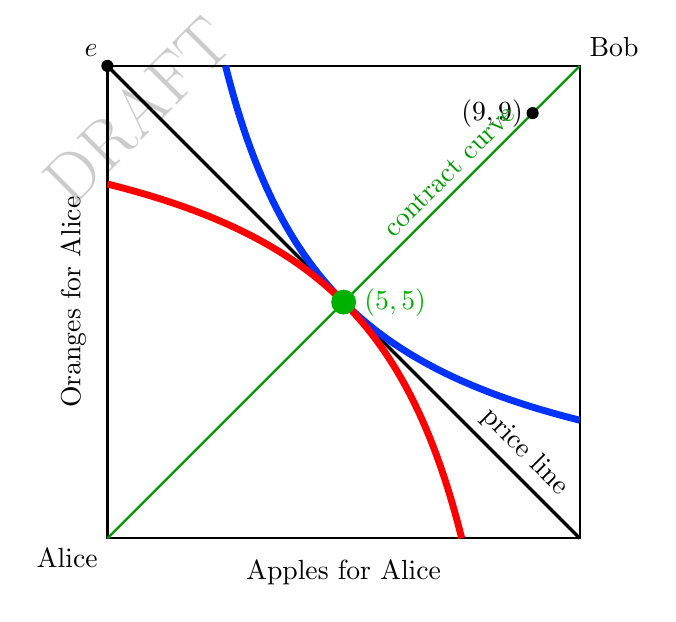
\begin{tikzpicture}[x=0.6cm,y=0.6cm]
  % Box
  \draw[thick] (0,0) rectangle (10,10);
  
  % Contract curve
  \draw[green!60!black, thick] (0,0)--(10,10);
  
  % Price line (black and thick to match the reference image)
  \draw[black, very thick] (0,10)--(10,0);
  
  % Alice's Indifference Curve (Blue)
  % Equation: y = 25/x, perfectly tangent to the price line at (5,5)
  \draw[blue!80!cyan, line width=2.5pt, domain=2.5:10, samples=100] plot (\x, {25/\x});
  
  % Bob's Indifference Curve (Red)
  % Equation: y = 10 - 25/(10-x), perfectly tangent to the price line at (5,5)
  \draw[red, line width=2.5pt, domain=0:7.5, samples=100] plot (\x, {10 - 25/(10-\x)});
  
  % Points
  \fill (0,10) circle (2.2pt) node[above left] {$e$};
  \fill (9,9) circle (2.2pt) node[left] {$(9,9)$};
  
  % Tangency Point
  \fill[green!70!black] (5,5) circle (4.5pt) node[right=4pt, font=\bfseries] {$(5,5)$};
  
  % Agent Labels
  \node[below left] at (0,0) {Alice};
  \node[above right] at (10,10) {Bob};
  
  % Rotated Line Labels (Aligns parallel to the lines for a cleaner look)
  \node[green!60!black, rotate=45, above] at (7.5,7.5) {contract curve};
  \node[rotate=-45, above] at (8.5,1.5) {price line};
  
  % Axis Labels (added spacing so they don't clip the box)
  \node[below=0.15cm] at (5,0) {Apples for Alice};
  \node[rotate=90, above=0.15cm] at (0,5) {Oranges for Alice};
\end{tikzpicture}
\end{center}
    \item
    At the allocation
    \[
    (A_A,O_A)=(9,9),\qquad (A_B,O_B)=(1,1),
    \]
    Alice's marginal rate of substitution is
    \[
    MRS_A=\frac{O_A}{A_A}=\frac{9}{9}=1,
    \]
    while Bob's marginal rate of substitution is
    \[
    MRS_B=\frac{O_B}{A_B}=\frac{1}{1}=1.
    \]
    Since the MRS values are equal, their indifference curves are tangent at that allocation. Therefore there is no local Pareto improvement.

    Equivalently, the allocation lies on the diagonal
    \[
    O_A=A_A,
    \]
    which is the interior contract curve for this economy. Hence it is Pareto efficient.

    Therefore
    \[
    \boxed{(9,9)\text{ for Alice and }(1,1)\text{ for Bob is Pareto efficient.}}
    \]

    \item
    At the competitive equilibrium from part (c), prices satisfy
    \[
    P_A=P_O.
    \]
    The supporting price line through \((5,5)\) is therefore
    \[
    P_A A_A + P_O O_A = 10P
    \qquad\Longrightarrow\qquad
    A_A+O_A=10.
    \]
    Any redistribution of the original endowment that lies on this line yields the same competitive equilibrium allocation \((5,5)\) after trading, because the equilibrium prices are unchanged and the equilibrium bundle remains on the same supporting budget line.

    Two examples are:
    \[
    \boxed{(A_A,O_A)=(7,3)}
    \qquad\text{and}\qquad
    \boxed{(A_A,O_A)=(3,7).}
    \]
    In each case, Bob receives the remaining bundle:
    \[
    (A_B,O_B)=(3,7)\quad\text{or}\quad (7,3),
    \]
    respectively.
\end{enumerate}

\newpage
\subsubsection{Method 2: Lagrangian derivation and contract-curve argument}

\begin{enumerate}[label=(\alph*)]
    \item
    We derive each consumer's demand from first principles.

    \paragraph{Alice.}
    Alice solves
    \[
    \max_{A_A,O_A\ge 0}\; A_A^{1/2}O_A^{1/2}
    \quad\text{subject to}\quad
    P_AA_A+P_OO_A=10P_O.
    \]
    The Lagrangian is
    \[
    \mathcal L=A_A^{1/2}O_A^{1/2}+\lambda(10P_O-P_AA_A-P_OO_A).
    \]
    The first-order conditions are
    \begin{align*}
        \frac{\partial\mathcal L}{\partial A_A}
        &=\frac12 A_A^{-1/2}O_A^{1/2}-\lambda P_A=0,\\
        \frac{\partial\mathcal L}{\partial O_A}
        &=\frac12 A_A^{1/2}O_A^{-1/2}-\lambda P_O=0.
    \end{align*}
    Dividing the first equation by the second gives
    \[
    \frac{O_A}{A_A}=\frac{P_A}{P_O}.
    \]
    Rearranging,
    \[
    P_OO_A=P_AA_A.
    \]
    Substitute into the budget constraint:
    \[
    P_AA_A+P_AA_A=10P_O,
    \]
    so
    \[
    2P_AA_A=10P_O
    \qquad\Longrightarrow\qquad
    A_A=\frac{5P_O}{P_A}.
    \]
    Then
    \[
    O_A=\frac{P_A}{P_O}A_A=5.
    \]

    \paragraph{Bob.}
    Bob solves
    \[
    \max_{A_B,O_B\ge 0}\; A_B^{1/2}O_B^{1/2}
    \quad\text{subject to}\quad
    P_AA_B+P_OO_B=10P_A.
    \]
    By the same steps,
    \[
    P_AA_B=P_OO_B.
    \]
    Substituting into the budget gives
    \[
    2P_AA_B=10P_A
    \qquad\Longrightarrow\qquad
    A_B=5,
    \]
    and then
    \[
    O_B=\frac{P_A}{P_O}A_B=\frac{5P_A}{P_O}.
    \]

    Hence
    \[
    \boxed{
    A_A=\frac{5P_O}{P_A},\quad O_A=5,\qquad A_B=5,\quad O_B=\frac{5P_A}{P_O}.}
    \]

    \item
    Market clearing requires
    \[
    A_A+A_B=10,\qquad O_A+O_B=10.
    \]
    Substituting the demand functions:
    \[
    \frac{5P_O}{P_A}+5=10
    \qquad\Longrightarrow\qquad
    P_O=P_A,
    \]
    and likewise
    \[
    5+\frac{5P_A}{P_O}=10
    \qquad\Longrightarrow\qquad
    P_O=P_A.
    \]
    Therefore
    \[
    \boxed{P_O=P_A.}
    \]

    \item
    The contract curve in the interior of the Edgeworth box is obtained by equating marginal rates of substitution:
    \[
    \frac{O_A}{A_A}=\frac{O_B}{A_B}.
    \]
    Feasibility implies
    \[
    A_B=10-A_A,\qquad O_B=10-O_A.
    \]
    Therefore
    \[
    \frac{O_A}{A_A}=\frac{10-O_A}{10-A_A}.
    \]
    Cross-multiplying,
    \[
    O_A(10-A_A)=A_A(10-O_A).
    \]
    Expanding both sides,
    \[
    10O_A-O_AA_A=10A_A-O_AA_A,
    \]
    so
    \[
    10O_A=10A_A
    \qquad\Longrightarrow\qquad
    \boxed{O_A=A_A.}
    \]
    Thus the contract curve is the main diagonal.

    In a competitive equilibrium, the price line through Alice's endowment \((0,10)\) has slope
    \[
    -\frac{P_A}{P_O}.
    \]
    Since market clearing gives \(P_A=P_O\), that slope is \(-1\), so the price line is
    \[
    A_A+O_A=10.
    \]
    Intersect this with the contract curve \(O_A=A_A\):
    \[
    A_A+A_A=10
    \qquad\Longrightarrow\qquad
    A_A=5.
    \]
    Hence
    \[
    O_A=5.
    \]
    Therefore
    \[
    \boxed{(A_A,O_A)=(5,5),\qquad (A_B,O_B)=(5,5).}
    \]

    \item
    The allocation \((9,9)\) for Alice gives Bob \((1,1)\). Both lie on the contract curve
    \[
    O_A=A_A.
    \]
    Therefore it is Pareto efficient. Equivalently,
    \[
    MRS_A=\frac{9}{9}=1=MRS_B=\frac{1}{1}.
    \]
    Hence
    \[
    \boxed{(9,9)\text{ for Alice and }(1,1)\text{ for Bob is Pareto efficient.}}
    \]

    \item
    The supporting price line through the competitive equilibrium is
    \[
    A_A+O_A=10.
    \]
    Any redistributed endowment on this line supports the same competitive equilibrium allocation after trade. For example,
    \[
    \boxed{(7,3)\quad\text{and}\quad (3,7)}
    \]
    for Alice, with Bob receiving the remaining goods in each case.
\end{enumerate}

%====================================================
% QUESTION 2
%====================================================
\newpage
\section{Question 2: Linus Straight and Lucy Kink}

\noindent
Linus Straight's utility function is \(U(a,b)=a+2b\), where \(a\) is his consumption of apples and \(b\) is his consumption of bananas. Lucy Kink's utility function is \(U(a,b)=\min\{a,2b\}\). Lucy has 12 apples and no bananas. Linus has 12 bananas and no apples.

\subsection{Problem}
\begin{enumerate}[label=(\alph*)]
    \item Draw an Edgeworth box, showing their endowment and draw (as accurately as possible) a few indifference curves for Lucy and Linus. Measure Lucy's consumption from the upper right corner and Linus's from the lower left corner.
    \item Draw the contract curve for this economy (the set of all Pareto Efficient allocations).

    Hint: given the shapes of the indifference curves you have drawn, at which points are there no area of pareto improvement?
    \item In this economy, show that if \(\dfrac{P_a}{P_b}\neq \dfrac12\), then there will always be excess demand of one of the goods.
    \item The previous part implies that in a competitive equilibrium, we must have \(\dfrac{P_a}{P_b}=\dfrac12\). Find the quantities of apples and bananas consumed in competitive equilibrium by Linus and Lucy.
\end{enumerate}

\newpage
\subsection{Solution}

\subsubsection{Method 1: Demand correspondences and market-clearing}

\begin{enumerate}[label=(\alph*)]
    \item
    Linus has utility
    \[
    U_L(a_L,b_L)=a_L+2b_L.
    \]
    His indifference curves satisfy
    \[
    a_L+2b_L=\bar U,
    \]
    or equivalently
    \[
    b_L=\frac{\bar U}{2}-\frac{a_L}{2}.
    \]
    Hence Linus's indifference curves are straight lines with slope
    \[
    -\frac12.
    \]

    Lucy has utility
    \[
    U_U(a_U,b_U)=\min\{a_U,2b_U\}.
    \]
    So her indifference curves are L-shaped, with kinks at bundles satisfying
    \[
    a_U=2b_U.
    \]

    If we draw the Edgeworth box using Linus's coordinates \((a_L,b_L)\) from the lower-left corner, then Lucy's consumption is
    \[
    a_U=12-a_L,\qquad b_U=12-b_L.
    \]
    Thus Lucy's kink condition becomes
    \[
    12-a_L=2(12-b_L),
    \]
    which simplifies to
    \[
    \boxed{b_L=6+\frac12 a_L.}
    \]

    The initial endowment is
    \[
    e=(a_L,b_L)=(0,12),
    \]
    since Linus owns 12 bananas and no apples.

    A correct schematic Edgeworth box is shown below.

\begin{center}
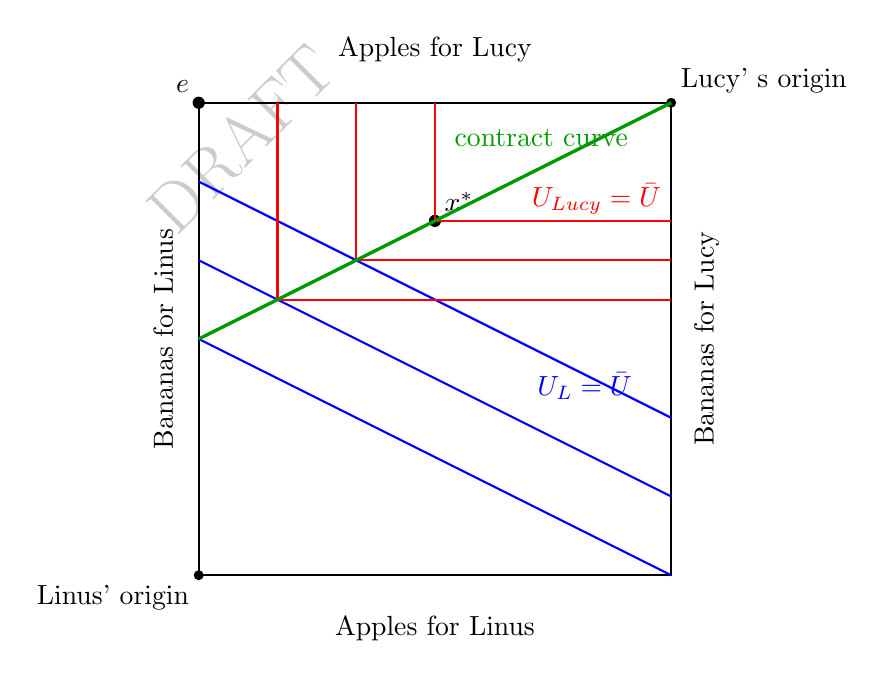
\begin{tikzpicture}[x=0.5cm,y=0.5cm]
  % Edgeworth box
  \draw[thick] (0,0) rectangle (12,12);

  % Origins
  \fill (0,0) circle (1.8pt);
  \fill (12,12) circle (1.8pt);
  \node[below left] at (0,0) {Linus' origin};
  \node[above right] at (12,12) {Lucy' s origin};

  % Endowment and CE
  \fill (0,12) circle (2.2pt) node[above left] {$e$};
  \fill (6,9) circle (2.2pt) node[above right] {$x^*$};

  % Linus indifference curves: a_L + 2b_L = U
  \draw[blue, thick] (0,10) -- (12,4);
  \draw[blue, thick] (0,8)  -- (12,2);
  \draw[blue, thick] (0,6)  -- (12,0);

  % Lucy indifference curves in Linus coordinates:
  % a_U = 12-a_L, b_U = 12-b_L, kink locus b_L = 6 + a_L/2
  \draw[red, thick] (2,12) -- (2,7) -- (12,7);
  \draw[red, thick] (4,12) -- (4,8) -- (12,8);
  \draw[red, thick] (6,12) -- (6,9) -- (12,9);

  % Contract curve
  \draw[green!60!black, very thick] (0,6) -- (12,12);

  % Labels
  \node[blue] at (9.8,4.8) {$U_L=\bar U$};
  \node[red] at (10.1,9.55) {$U_{Lucy}=\bar U$};
  \node[green!60!black] at (8.7,11.1) {contract curve};

  % Axis labels
  \node[below] at (6,-0.8) {Apples for Linus};
  \node[rotate=90] at (-0.9,6) {Bananas for Linus};
  \node[above] at (6,12.8) {Apples for Lucy};
  \node[rotate=90] at (12.9,6) {Bananas for Lucy};


\end{tikzpicture}
\end{center}

    \item
    A Pareto efficient allocation must leave Lucy with no redundant amount of one good relative to the other. If Lucy has
    \[
    a_U>2b_U,
    \]
    then some apples are slack for her utility: decreasing apples slightly does not reduce
    \[
    U_U(a_U,b_U)=\min\{a_U,2b_U\}=2b_U.
    \]
    Those apples can be transferred to Linus, making Linus strictly better off while Lucy is unchanged.

    Similarly, if
    \[
    a_U<2b_U,
    \]
    then some bananas are slack for Lucy. A small reduction in bananas leaves Lucy's utility unchanged, and the bananas can be transferred to Linus, again yielding a Pareto improvement.

    Therefore at any Pareto efficient allocation Lucy must be exactly at her kink:
    \[
    \boxed{a_U=2b_U.}
    \]

    In Lucy's own coordinates this is the contract curve. In Linus's coordinates it becomes
    \[
    \boxed{b_L=6+\frac12 a_L.}
    \]

\newpage
    \item
    Let \(P_a\) denote the price of apples and \(P_b\) the price of bananas.

    Linus owns 12 bananas, so his wealth is
    \[
    m_L=12P_b.
    \]
    His utility is
    \[
    U_L(a_L,b_L)=a_L+2b_L,
    \]
    so the marginal utility per dollar of apples is
    \[
    \frac{MU_a}{P_a}=\frac{1}{P_a},
    \]
    while the marginal utility per dollar of bananas is
    \[
    \frac{MU_b}{P_b}=\frac{2}{P_b}.
    \]

    \paragraph{Case 1: \(\dfrac{P_a}{P_b}>\dfrac12\).}
    Then
    \[
    \frac{1}{P_a}<\frac{2}{P_b}.
    \]
    Bananas give higher marginal utility per dollar, so Linus demands only bananas. Since he can afford
    \[
    b_L=\frac{m_L}{P_b}=\frac{12P_b}{P_b}=12,
    \]
    his demand is
    \[
    (a_L,b_L)=(0,12).
    \]

    Lucy has wealth
    \[
    m_U=12P_a>0.
    \]
    Because Lucy has perfect complements preferences, her optimal bundle must satisfy
    \[
    a_U=2b_U.
    \]
    Therefore she must demand a positive quantity of bananas:
    \[
    b_U>0.
    \]
    But the total supply of bananas is only 12, and Linus already demands all 12 bananas. Hence banana demand strictly exceeds banana supply.

    Therefore there is excess demand for bananas.

    \paragraph{Case 2: \(\dfrac{P_a}{P_b}<\dfrac12\).}
    Then
    \[
    \frac{1}{P_a}>\frac{2}{P_b}.
    \]
    Apples give higher marginal utility per dollar, so Linus demands only apples. Since his wealth is \(12P_b\), his apple demand is
    \[
    a_L=\frac{12P_b}{P_a}.
    \]
    Because
    \[
    \frac{P_a}{P_b}<\frac12
    \qquad\Longrightarrow\qquad
    \frac{P_b}{P_a}>2,
    \]
    we have
    \[
    a_L=12\frac{P_b}{P_a}>24.
    \]
    Yet total supply of apples is only 12. Hence there is excess demand for apples.

    Therefore, if
    \[
    \frac{P_a}{P_b}\neq \frac12,
    \]
    there is always excess demand for one of the two goods. So we have shown
    \[
    \boxed{\frac{P_a}{P_b}\neq \frac12 \;\Longrightarrow\; \text{excess demand for one good}.}
    \]

    \item
    From part (c), a competitive equilibrium requires
    \[
    \boxed{\frac{P_a}{P_b}=\frac12.}
    \]

    Lucy's wealth is
    \[
    m_U=12P_a.
    \]
    Since her utility is \(\min\{a_U,2b_U\}\), she chooses a bundle on the kink:
    \[
    a_U=2b_U.
    \]
    Her budget constraint is
    \[
    P_a a_U + P_b b_U = 12P_a.
    \]
    Substitute \(P_a=\frac12 P_b\):
    \[
    \frac12 P_b a_U + P_b b_U = 6P_b.
    \]
    Divide through by \(P_b\):
    \[
    \frac12 a_U+b_U=6.
    \]
    Together with \(a_U=2b_U\), this gives
    \[
    \frac12(2b_U)+b_U=6
    \qquad\Longrightarrow\qquad
    2b_U=6
    \qquad\Longrightarrow\qquad
    b_U=3.
    \]
    Hence
    \[
    a_U=2b_U=6.
    \]
    Therefore Lucy consumes
    \[
    \boxed{(a_U,b_U)=(6,3).}
    \]

    Linus then consumes the remaining bundle:
    \[
    a_L=12-6=6,\qquad b_L=12-3=9.
    \]
    So
    \[
    \boxed{(a_L,b_L)=(6,9).}
    \]

    We can verify that Linus is willing to choose this bundle. At \(\frac{P_a}{P_b}=\frac12\), his budget line is
    \[
    P_a a_L+P_b b_L=12P_b
    \qquad\Longleftrightarrow\qquad
    \frac12 a_L+b_L=12.
    \]
    Multiplying by 2 gives
    \[
    a_L+2b_L=24.
    \]
    Since Linus's utility is also \(a_L+2b_L\), every affordable bundle on this budget line gives the same utility. In particular,
    \[
    6+2(9)=24,
    \]
    so \((6,9)\) is utility-maximising for Linus.

    Hence the competitive equilibrium allocation is
    \[
    \boxed{\text{Lucy consumes }(6,3),\qquad \text{Linus consumes }(6,9).}
    \]
\end{enumerate}

\newpage
\subsubsection{Method 2: Geometry of price lines and the contract curve}

\begin{enumerate}[label=(\alph*)]
    \item
    The geometry is immediate from the utilities.

    Linus has perfect substitutes preferences, so each indifference curve is a straight line with slope
    \[
    -\frac{MU_a}{MU_b}=-\frac{1}{2}.
    \]
    Lucy has perfect complements preferences, so each indifference curve is an L-shape with kinks along
    \[
    a_U=2b_U.
    \]
    In the Edgeworth box measured from Linus's origin, this kink locus is
    \[
    b_L=6+\frac12 a_L.
    \]

    \item
    The contract curve is exactly Lucy's kink locus:
    \[
    \boxed{a_U=2b_U.}
    \]
    Any point off this locus leaves Lucy with slack of one good, and that slack can be reassigned to Linus without hurting Lucy. Hence only the kink locus can be Pareto efficient.

    \item
    In the Edgeworth box, the competitive budget line has slope
    \[
    -\frac{P_a}{P_b}.
    \]
    Linus's indifference curves have slope
    \[
    -\frac12.
    \]

    \paragraph{If \(\dfrac{P_a}{P_b}>\dfrac12\).}
    The budget line is steeper than Linus's indifference curves. Linus therefore maximises utility at the banana corner of his budget set, so he demands only bananas. Since Lucy must also demand bananas to attain positive utility, there is excess demand for bananas.

    \paragraph{If \(\dfrac{P_a}{P_b}<\dfrac12\).}
    The budget line is flatter than Linus's indifference curves. Linus therefore chooses the apple corner of his budget set, so he demands only apples. Because his wealth is 12 bananas, his apple demand exceeds the total supply of apples, so there is excess demand for apples.

    Hence a competitive equilibrium can exist only if
    \[
    \boxed{\frac{P_a}{P_b}=\frac12.}
    \]

    \item
    Once
    \[
    \frac{P_a}{P_b}=\frac12,
    \]
    Linus's budget line is parallel to his indifference curves, so he is indifferent among all affordable bundles. The competitive allocation must therefore be determined by Lucy's optimal choice together with market clearing.

    Lucy's budget line through her endowment has value
    \[
    12P_a.
    \]
    Her optimum occurs where this price line meets her kink line
    \[
    a_U=2b_U.
    \]
    Writing the budget as
    \[
    P_a a_U + P_b b_U = 12P_a
    \]
    and substituting \(P_a/P_b=1/2\), we get
    \[
    \frac12 a_U+b_U=6.
    \]
    Together with \(a_U=2b_U\), this gives
    \[
    (a_U,b_U)=(6,3).
    \]
    Feasibility then implies
    \[
    (a_L,b_L)=(12-6,\,12-3)=(6,9).
    \]

    Therefore
    \[
    \boxed{\text{Lucy consumes }(6,3),\qquad \text{Linus consumes }(6,9).}
    \]
\end{enumerate}

%====================================================
% QUESTION 3
%====================================================
\newpage
\section{Question 3: Paul, David, Envy, and Fairness}

\noindent
Paul and David consume apples and oranges. Paul's utility function is \(U_P(A_P,O_P)=2A_P+O_P\) and David's utility function is \(U_D(A_D,O_D)=A_D+2O_D\), where \(A_P\) and \(A_D\) are apple consumptions for Paul and David, and \(O_P\) and \(O_D\) are orange consumptions for Paul and David.

\noindent
There are a total of 12 apples and 12 oranges to divide between Paul and David.

\subsection{Problem}
\begin{enumerate}[label=(\alph*)]
    \item Draw an Edgeworth box showing the indifference curves for Paul and David passing through each of the points A to E. Explain whether each of the points A to E is Pareto Efficient.

% ============================================================
% Blank graph (for drawing)
% ============================================================
\begin{center}
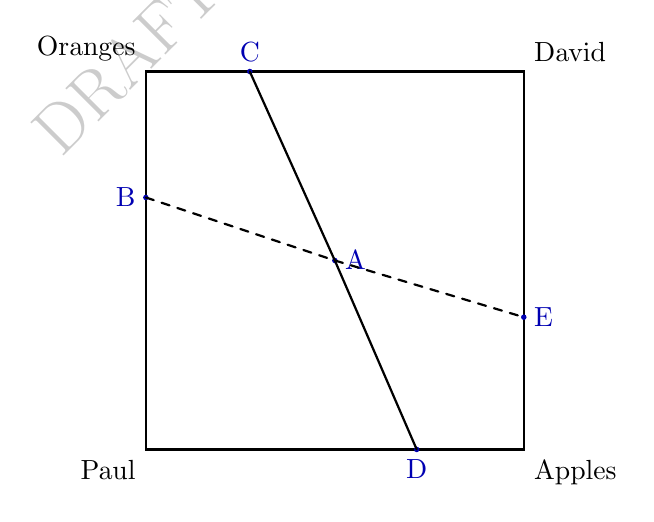
\begin{tikzpicture}[
    scale=0.4, % Increase scale for a better zoomed-in view
    >=latex,
    thick,
    line cap=round,
    label style/.style={font=\small}
]
  % Edgeworth box
  \draw[thick] (0,0) rectangle (12,12);

  % Boundary points (B, C, D, E on edges)
  \fill[blue!70!black] (0,8) circle (2.5pt) node[left] {B};
  \fill[blue!70!black] (3.3,12) circle (2.5pt) node[above] {C};
  \fill[blue!70!black] (8.6,0) circle (2.5pt) node[below] {D};
  \fill[blue!70!black] (12,4.2) circle (2.5pt) node[right] {E};

  % Interior point A
  \fill[blue!70!black] (6,6) circle (2.5pt) node[right] {A};

  % Lines: C-A-D (slope -2), B-A-E (slope -1/2)
  \draw[thick] (3.3,12) -- (6,6) -- (8.6,0);
  \draw[thick,dashed] (0,8) -- (6,6) -- (12,4.2);

  % Labels
  \node[above left] at (0,12) {Oranges};
  \node[below left] at (0,0) {Paul};
  \node[above right] at (12,12) {David};
  \node[below right] at (12,0) {Apples};
\end{tikzpicture}
\end{center}

    (To make the drawing simpler, you can assume for simplicity that the points are such that C,A,D form a straight line with slope \(-2\) while B,A,E form a straight line with slope \(-1/2\))
    \item Using your answer in (a), draw the contract curve (the set of all Pareto Efficient allocations) in the Edgeworth Box.
    \item Derive the set of envy-free allocations using the following procedure.
    \begin{enumerate}[label=\Roman*.]
        \item Write one inequality that says that Paul likes his own bundle \((A_P,O_P)\) as well as much as he likes David's \((A_D,O_D)\).
        \item Write another inequality that says that David likes his own bundle \((A_D,O_D)\) as much as he likes Paul's \((A_P,O_P)\).
        \item Use the fact that at feasible allocations, \(A_P + A_D = 12\) and \(O_P + O_D =12\) to rewrite the above inequalities in terms of \(A_P\) and \(O_P\) for both Paul and David.
        \item Indicate the set of allocations which satisfy both of these inequalities in the figure.
    \end{enumerate}
    \item In the Edgeworth box, denote the set of fair allocations.
\end{enumerate}

\newpage
\subsection{Solution}

\subsubsection{Method 1: Pareto-improvement directions and envy inequalities}

\begin{enumerate}[label=(\alph*)]
    \item
    Paul's indifference curves satisfy
    \[
    2A_P+O_P=\bar U_P
    \qquad\Longleftrightarrow\qquad
    O_P=\bar U_P-2A_P.
    \]
    So their slope is
    \[
    -2.
    \]

    David's indifference curves satisfy
    \[
    A_D+2O_D=\bar U_D
    \qquad\Longleftrightarrow\qquad
    O_D=\frac{\bar U_D}{2}-\frac{A_D}{2},
    \]
    so in David's own coordinates their slope is
    \[
    -\frac12.
    \]

    A suitable is shown below.

\begin{center}
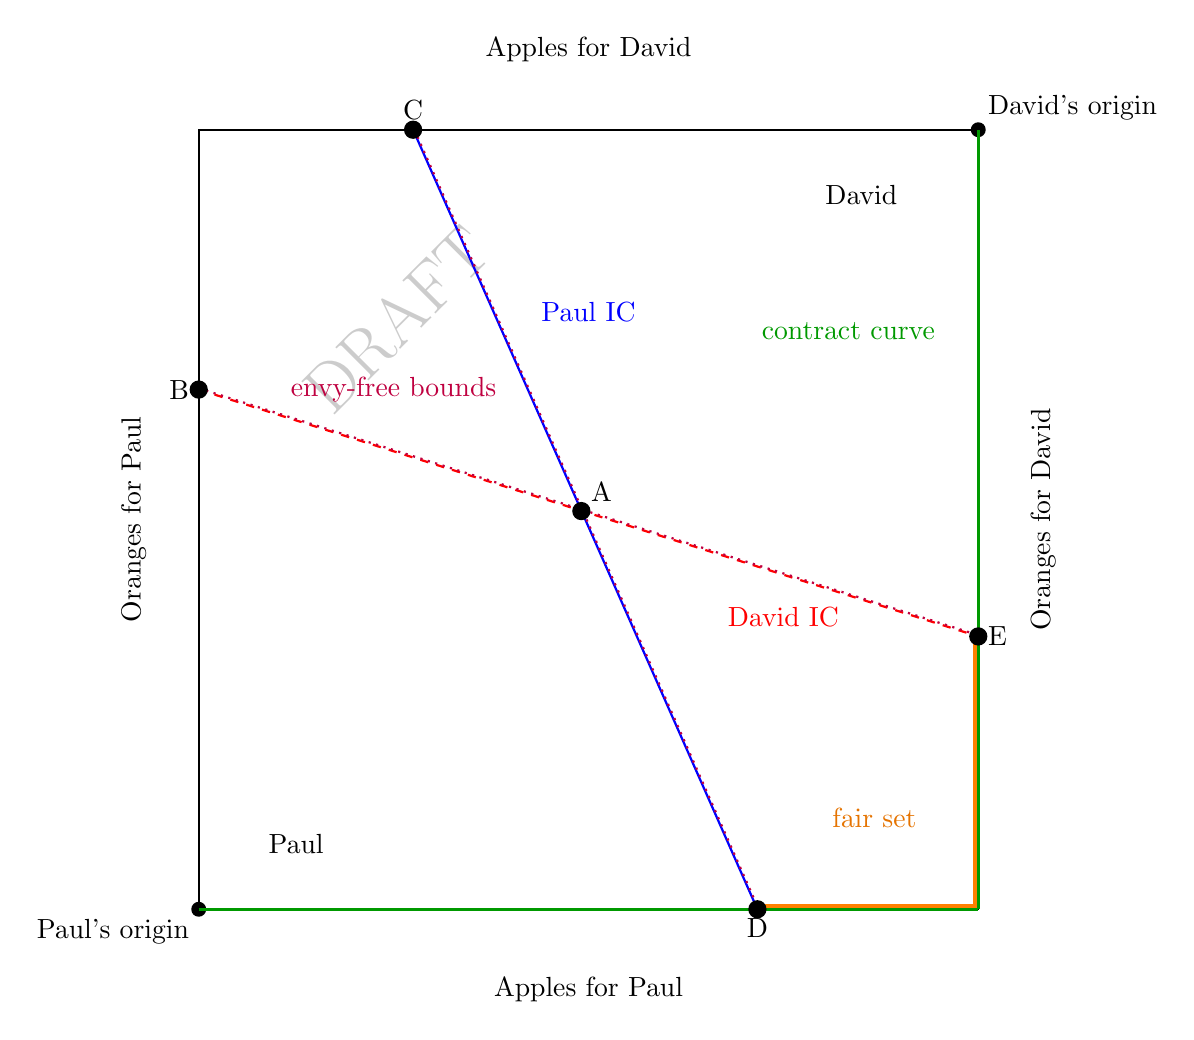
\begin{tikzpicture}[scale=1.5, x=0.55cm,y=0.55cm]
  % Edgeworth box
  \draw[thick] (0,0) rectangle (12,12);

  % Origins
  \fill (0,0) circle (1.8pt);
  \fill (12,12) circle (1.8pt);
  \node[below left] at (0,0) {Paul's origin};
  \node[above right] at (12,12) {David's origin};

  % Contract curve
  \draw[green!60!black, very thick] (0,0) -- (12,0);
  \draw[green!60!black, very thick] (12,0) -- (12,12);

  % Main reference lines
  \draw[blue, thick] (3.3,12) -- (8.6,0);            % C-A-D line
  \draw[red, dashed, thick] (0,8) -- (12,4.2);       % B-A-E line

  % Envy-free boundary lines
  \draw[purple, dotted, thick] (3.32,12) -- (8.62,0);
  \draw[purple, dotted, thick] (0,8.02) -- (12,4.22);

  % Fair set
  \draw[orange, ultra thick] (8.6,0.05) -- (11.95,0.05);
  \draw[orange, ultra thick] (11.95,0.02) -- (11.95,4.2);

  % Points
  \fill (5.89,6.13) circle (2.2pt) node[above right] {A};
  \fill (0,8) circle (2.2pt) node[left] {B};
  \fill (3.3,12) circle (2.2pt) node[above] {C};
  \fill (8.6,0) circle (2.2pt) node[below] {D};
  \fill (12,4.2) circle (2.2pt) node[right] {E};

  % Labels
  \node[blue] at (6,9.2) {Paul IC};
  \node[red] at (9.0,4.5) {David IC};
  \node[green!60!black] at (10.0,8.9) {contract curve};
  \node[purple] at (3,8) {envy-free bounds};
  \node[orange!90!black] at (10.4,1.4) {fair set};

  % Axis labels
  \node[below] at (6,-0.9) {Apples for Paul};
  \node[rotate=90] at (-1.0,6) {Oranges for Paul};
  \node[above] at (6,12.9) {Apples for David};
  \node[rotate=90] at (13.0,6) {Oranges for David};

  % Consumer names
  \node at (1.5,1.0) {Paul};
  \node at (10.2,11.0) {David};
\end{tikzpicture}
\end{center}
    
% ============================================================
% Filled graph (corrected)
% ============================================================




    To test Pareto efficiency, consider any interior feasible allocation \((A_P,O_P)\) with
    \[
    0<A_P<12,\qquad 0<O_P<12.
    \]
    Suppose we move slightly in the south-east direction:
    \[
    \Delta A_P=\varepsilon>0,\qquad \Delta O_P=-\eta<0.
    \]
    Then Paul's utility changes by
    \[
    \Delta U_P = 2\varepsilon-\eta.
    \]
    David receives the opposite change:
    \[
    \Delta A_D=-\varepsilon,\qquad \Delta O_D=\eta,
    \]
    so David's utility changes by
    \[
    \Delta U_D = -\varepsilon + 2\eta.
    \]
    If we choose \(\eta\) so that
    \[
    \frac{\varepsilon}{2}<\eta<2\varepsilon,
    \]
    then
    \[
    \Delta U_P>0
    \qquad\text{and}\qquad
    \Delta U_D>0.
    \]
    Therefore every interior point is Pareto inefficient.

    Since the solution sheet identifies A, B, and C as interior points of this type, they are not Pareto efficient. By contrast, D lies on the bottom border and E lies on the right border. At such points, there is no feasible south-east move remaining inside the Edgeworth box, so no Pareto improvement is possible.

    Hence
    \[
    \boxed{\text{A, B, and C are not Pareto efficient, while D and E are Pareto efficient.}}
    \]

    \item
    From the argument above, every interior point is Pareto inefficient. The only candidates are points where the south-east Pareto-improvement direction is blocked by feasibility, namely:
    \begin{itemize}[leftmargin=*]
        \item the bottom border, where \(O_P=0\);
        \item the right border, where \(A_P=12\).
    \end{itemize}
    Therefore the contract curve is
    \[
    \boxed{\mathcal C
    =\{(A_P,O_P): O_P=0,\ 0\le A_P\le 12\}
    \cup
    \{(A_P,O_P): A_P=12,\ 0\le O_P\le 12\}.}
    \]

    \item
    \paragraph{I. Paul's no-envy inequality.}
    Paul weakly prefers his own bundle to David's if
    \[
    U_P(A_P,O_P)\ge U_P(A_D,O_D).
    \]
    Using his utility function,
    \[
    2A_P+O_P\ge 2A_D+O_D.
    \]

    \paragraph{II. David's no-envy inequality.}
    David weakly prefers his own bundle to Paul's if
    \[
    U_D(A_D,O_D)\ge U_D(A_P,O_P).
    \]
    Using his utility function,
    \[
    A_D+2O_D\ge A_P+2O_P.
    \]

    \paragraph{III. Rewrite using feasibility.}
    Since
    \[
    A_D=12-A_P,\qquad O_D=12-O_P,
    \]
    Paul's inequality becomes
    \begin{align*}
        2A_P+O_P &\ge 2(12-A_P)+(12-O_P)\\
        2A_P+O_P &\ge 36-2A_P-O_P\\
        4A_P+2O_P &\ge 36\\
        2A_P+O_P &\ge 18.
    \end{align*}
    So Paul's no-envy region is
    \[
    \boxed{O_P\ge 18-2A_P.}
    \]

    David's inequality becomes
    \begin{align*}
        (12-A_P)+2(12-O_P) &\ge A_P+2O_P\\
        36-A_P-2O_P &\ge A_P+2O_P\\
        36 &\ge 2A_P+4O_P\\
        18 &\ge A_P+2O_P.
    \end{align*}
    So David's no-envy region is
    \[
    \boxed{O_P\le 9-\frac{A_P}{2}.}
    \]

    \paragraph{IV. Envy-free allocations.}
    An allocation is envy-free if both inequalities hold simultaneously. Therefore the envy-free set is
    \[
    \boxed{\mathcal E
    =\left\{(A_P,O_P):
    O_P\ge 18-2A_P,\;
    O_P\le 9-\frac{A_P}{2},\;
    0\le A_P\le 12,\;
    0\le O_P\le 12
    \right\}.}
    \]

    A schematic figure is shown below.

    \begin{center}
    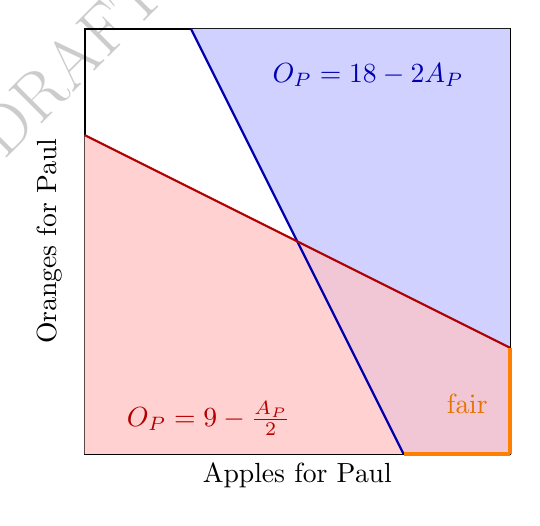
\begin{tikzpicture}[x=0.45cm,y=0.45cm]
      \draw[thick] (0,0) rectangle (12,12);

      % Regions
      \fill[blue!18] (3,12)--(12,12)--(12,0)--(9,0)--cycle;
      \fill[red!18] (0,0)--(0,9)--(12,3)--(12,0)--cycle;
      \fill[purple!22] (6,6)--(12,3)--(12,0)--(9,0)--cycle;

      % Boundary lines
      \draw[blue!70!black, thick] (3,12)--(9,0);
      \draw[red!70!black, thick] (0,9)--(12,3);

      % Fair set on contract curve
      \draw[orange, ultra thick] (9,0)--(12,0);
      \draw[orange, ultra thick] (12,0)--(12,3);

      \node[blue!70!black] at (8,10.7) {$O_P=18-2A_P$};
      \node[red!70!black] at (3.5,1) {$O_P=9-\frac{A_P}{2}$};
      \node[orange!90!black] at (10.8,1.4) {fair};
      \node[below] at (6,0) {Apples for Paul};
      \node[rotate=90] at (-1.0,6) {Oranges for Paul};
    \end{tikzpicture}
    \end{center}

    \item
    A fair allocation is both Pareto efficient and envy-free. Therefore
    \[
    \mathcal F=\mathcal C\cap\mathcal E.
    \]

    Intersect the envy-free set with each part of the contract curve.

    \paragraph{Bottom edge: \(O_P=0\).}
    Paul's no-envy condition gives
    \[
    0\ge 18-2A_P
    \qquad\Longrightarrow\qquad
    A_P\ge 9.
    \]
    David's no-envy condition gives
    \[
    0\le 9-\frac{A_P}{2}
    \qquad\Longrightarrow\qquad
    A_P\le 18,
    \]
    which is automatically true inside the box. So the fair part of the bottom edge is
    \[
    \{(A_P,0): 9\le A_P\le 12\}.
    \]

    \paragraph{Right edge: \(A_P=12\).}
    Paul's no-envy condition becomes
    \[
    O_P\ge 18-24=-6,
    \]
    which is automatic. David's no-envy condition becomes
    \[
    O_P\le 9-\frac{12}{2}=3.
    \]
    So the fair part of the right edge is
    \[
    \{(12,O_P): 0\le O_P\le 3\}.
    \]

    Therefore the set of fair allocations is
    \[
    \boxed{
    \mathcal F
    =
    \{(A_P,0): 9\le A_P\le 12\}
    \cup
    \{(12,O_P): 0\le O_P\le 3\}.}
    \]
\end{enumerate}

\subsubsection{Method 2: Weighted-sum characterisation of efficiency and boundary-by-boundary fairness}

\begin{enumerate}[label=(\alph*)]
    \item
    Pareto efficient allocations can be found by maximising a weighted sum of utilities:
    \[
    \max_{A_P,O_P}\;
    \lambda U_P(A_P,O_P)+(1-\lambda)U_D(A_D,O_D),
    \qquad 0<\lambda<1,
    \]
    subject to
    \[
    A_D=12-A_P,\qquad O_D=12-O_P.
    \]
    Substituting the utility functions,
    \begin{align*}
        W(A_P,O_P)
        &=\lambda(2A_P+O_P)+(1-\lambda)\bigl((12-A_P)+2(12-O_P)\bigr)\\
        &=36(1-\lambda) + (3\lambda-1)A_P + (3\lambda-2)O_P.
    \end{align*}
    Since \(W\) is linear, the maximiser is always on the boundary of the box.

    Depending on \(\lambda\):
    \begin{itemize}[leftmargin=*]
        \item if \(\lambda<\tfrac13\), both coefficients are negative, so the maximiser lies at \((0,0)\);
        \item if \(\lambda=\tfrac13\), the coefficient on \(A_P\) is zero and the coefficient on \(O_P\) is negative, so any point on the bottom edge is optimal;
        \item if \(\tfrac13<\lambda<\tfrac23\), the coefficient on \(A_P\) is positive and the coefficient on \(O_P\) is negative, so the maximiser is \((12,0)\);
        \item if \(\lambda=\tfrac23\), the coefficient on \(A_P\) is positive and the coefficient on \(O_P\) is zero, so any point on the right edge is optimal;
        \item if \(\lambda>\tfrac23\), both coefficients are positive, so the maximiser is \((12,12)\).
    \end{itemize}
    Therefore all Pareto efficient allocations lie on the bottom or right edge. This confirms that D and E can be Pareto efficient, whereas interior points such as A, B, and C cannot.

    \item
    Thus the contract curve is
    \[
    \boxed{\mathcal C
    =\{(A_P,O_P): O_P=0,\ 0\le A_P\le 12\}
    \cup
    \{(A_P,O_P): A_P=12,\ 0\le O_P\le 12\}.}
    \]

    \item
    The no-envy inequalities are the same as in Method 1:
    \[
    2A_P+O_P\ge 2A_D+O_D,
    \qquad
    A_D+2O_D\ge A_P+2O_P.
    \]
    Using feasibility,
    \[
    A_D=12-A_P,\qquad O_D=12-O_P,
    \]
    these become
    \[
    \boxed{O_P\ge 18-2A_P}
    \qquad\text{and}\qquad
    \boxed{O_P\le 9-\frac{A_P}{2}.}
    \]
    Hence the envy-free set is
    \[
    \boxed{\mathcal E
    =\left\{(A_P,O_P):
    O_P\ge 18-2A_P,\;
    O_P\le 9-\frac{A_P}{2}\right\}
    \cap [0,12]^2.}
    \]

    \item
    To find fair allocations, intersect \(\mathcal E\) with the contract curve \(\mathcal C\).

    \paragraph{Bottom edge \(O_P=0\).}
    Envy-freeness requires
    \[
    0\ge 18-2A_P
    \qquad\Longrightarrow\qquad
    A_P\ge 9.
    \]
    So the fair bottom-edge segment is
    \[
    \{(A_P,0): 9\le A_P\le 12\}.
    \]

    \paragraph{Right edge \(A_P=12\).}
    Envy-freeness requires
    \[
    O_P\le 9-\frac{12}{2}=3.
    \]
    So the fair right-edge segment is
    \[
    \{(12,O_P): 0\le O_P\le 3\}.
    \]

    Therefore
    \[
    \boxed{
    \mathcal F
    =
    \{(A_P,0): 9\le A_P\le 12\}
    \cup
    \{(12,O_P): 0\le O_P\le 3\}.}
    \]
\end{enumerate}

%====================================================
% QUESTION 4
%====================================================
\newpage
\section{Question 4: Astrid and Birger}

\noindent
Consider a small exchange economy with two consumers, Astrid and Birger, and two commodities, herring and cheese. Astrid's initial endowment is 4 units of herring and 1 unit of cheese. Birger's initial endowment has no herring and 7 units of cheese. Astrid's utility function is \(U(H_A,C_A)=H_AC_A\). Birger is a more inflexible person. His utility function is \(U(H_B,C_B)=\min\{H_B,C_B\}\).

\noindent
(Here \(H_A\) and \(C_A\) are the amounts of herring and cheese for Astrid, and \(H_B\) and \(C_B\) are amounts of herring and cheese for Birger.)

\subsection{Problem}
\begin{enumerate}[label=(\alph*)]
    \item Draw an Edgeworth box, showing the initial allocation and sketching in a few indifference curves. Measure Astrid's consumption from the lower left and Birger's from the upper right. In your Edgeworth box, draw two different indifference curves for each person.
    \item Let cheese be the numeraire (with price 1) and let \(p\) denote the price of herring. Derive the allocations and prices in the competitive equilibrium. (Hint: follow the steps in the lecture and question 1)
    \item Sketch the competitive equilibrium in the Edgeworth Box.
\end{enumerate}

\newpage
\subsection{Solution}

\subsubsection{Method 1: Demand functions and market clearing}

\begin{enumerate}[label=(\alph*)]
    \item
    Total endowments are
    \[
    H_A+H_B=4,\qquad C_A+C_B=8.
    \]
    So the Edgeworth box has width 4 (herring) and height 8 (cheese) when measured from Astrid's origin at the lower left.

    Astrid's indifference curves satisfy
    \[
    H_A C_A = \bar U_A,
    \]
    so they are standard Cobb--Douglas hyperbolae.

    Birger's indifference curves satisfy
    \[
    \min\{H_B,C_B\}=\bar U_B,
    \]
    so they are L-shaped with kinks at
    \[
    H_B=C_B.
    \]
    In Astrid's coordinates, since
    \[
    H_B=4-H_A,\qquad C_B=8-C_A,
    \]
    Birger's kink locus becomes
    \[
    4-H_A = 8-C_A
    \qquad\Longrightarrow\qquad
    \boxed{C_A=H_A+4.}
    \]

    The initial allocation is
    \[
    e=(H_A,C_A)=(4,1).
    \]

    A correct sketch is shown below.
% --- Graph for part (a): Edgeworth box with initial allocation and indifference curves ---
\begin{center}
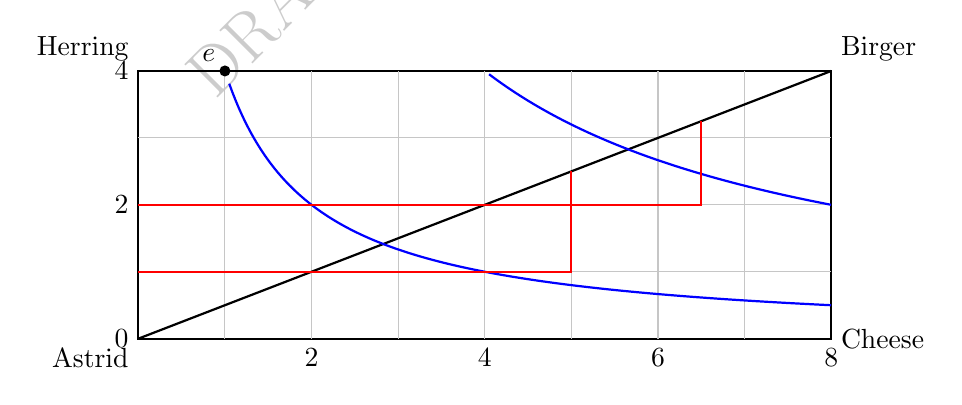
\begin{tikzpicture}[x=1.1cm,y=0.85cm]
  % Box
  \draw[thick] (0,0) rectangle (8,4);

  % Light grid
  \draw[gray!45, thin] (1,0) -- (1,4);
  \draw[gray!45, thin] (2,0) -- (2,4);
  \draw[gray!45, thin] (3,0) -- (3,4);
  \draw[gray!45, thin] (4,0) -- (4,4);
  \draw[gray!45, thin] (5,0) -- (5,4);
  \draw[gray!45, thin] (6,0) -- (6,4);
  \draw[gray!45, thin] (7,0) -- (7,4);

  \draw[gray!45, thin] (0,1) -- (8,1);
  \draw[gray!45, thin] (0,2) -- (8,2);
  \draw[gray!45, thin] (0,3) -- (8,3);

  % Axes labels / corner labels
  \node[above left] at (0,4) {Herring};
  \node[below left] at (0,0) {Astrid};
  \node[above right] at (8,4) {Birger};
  \node[right] at (8,0) {Cheese};

  % Tick labels (Astrid's coordinates)
  \node[left] at (0,0) {$0$};
  \node[left] at (0,2) {$2$};
  \node[left] at (0,4) {$4$};

  \node[below] at (2,0) {$2$};
  \node[below] at (4,0) {$4$};
  \node[below] at (6,0) {$6$};
  \node[below] at (8,0) {$8$};

  % Endowment
  \fill (1,4) circle (2pt);
  \node[above left] at (1,4) {$e$};

  % Birger kink locus: H_B = C_B  -> in Astrid coords y = x/2
  \draw[black, thick] (0,0) -- (8,4);

  % Astrid indifference curves H_A C_A = const
  \draw[blue, thick, domain=1.05:8, samples=200, smooth] plot (\x,{4/\x});
  \draw[blue, thick, domain=4.05:8, samples=200, smooth] plot (\x,{16/\x});

  % Birger L-shaped indifference curves
  \draw[red, thick] (0,1) -- (5,1) -- (5,2.5);
  \draw[red, thick] (0,2) -- (6.5,2) -- (6.5,3.25);

\end{tikzpicture}
\end{center}



    \item
    Let the price of cheese be normalised to 1, and let the price of herring be \(p\).

    \paragraph{Astrid's demand.}
    Astrid's wealth is the value of her endowment:
    \[
    m_A = 4p+1.
    \]
    Since her utility is
    \[
    U(H_A,C_A)=H_A C_A,
    \]
    she is Cobb--Douglas with equal exponents, so she spends one-half of her wealth on each good. Therefore
    \[
    pH_A = \frac12 (4p+1),\qquad C_A=\frac12 (4p+1).
    \]
    Thus
    \[
    \boxed{H_A=\frac{4p+1}{2p},\qquad C_A=\frac{4p+1}{2}.}
    \]

    \paragraph{Birger's demand.}
    Birger's wealth is
    \[
    m_B=7.
    \]
    Since his utility is \(\min\{H_B,C_B\}\), his optimal bundle satisfies
    \[
    H_B=C_B.
    \]
    If he consumes \(t\) units of each good, his budget is
    \[
    pt+t=7.
    \]
    Hence
    \[
    t=\frac{7}{p+1}.
    \]
    Therefore
    \[
    \boxed{H_B=C_B=\frac{7}{p+1}.}
    \]

    \paragraph{Market clearing.}
    Clear the herring market:
    \[
    H_A+H_B=4.
    \]
    So
    \[
    \frac{4p+1}{2p}+\frac{7}{p+1}=4.
    \]
    Multiply both sides by \(2p(p+1)\):
    \[
    (4p+1)(p+1)+14p = 8p(p+1).
    \]
    Expanding,
    \[
    4p^2+5p+1+14p = 8p^2+8p.
    \]
    Hence
    \[
    4p^2-11p-1=0.
    \]
    Solving the quadratic,
    \[
    p=\frac{11\pm \sqrt{121+16}}{8}
    =\frac{11\pm \sqrt{137}}{8}.
    \]
    Only the positive root is admissible, so
    \[
    \boxed{p^{*}=\frac{11+\sqrt{137}}{8}.}
    \]

    \paragraph{Equilibrium allocations.}
    Substitute \(p^{*}\) into Astrid's demand:
    \[
    H_A^{*}=\frac{4p^{*}+1}{2p^{*}}
    =\frac{\sqrt{137}-3}{4},
    \]
    and
    \[
    C_A^{*}=\frac{4p^{*}+1}{2}
    =\frac{\sqrt{137}+13}{4}.
    \]
    Birger then consumes
    \[
    H_B^{*}=4-H_A^{*}=\frac{19-\sqrt{137}}{4},
    \]
    and
    \[
    C_B^{*}=8-C_A^{*}=\frac{19-\sqrt{137}}{4}.
    \]

    Hence the competitive equilibrium is

    \begin{equation*}
    \boxed{
    \begin{aligned}
        p^{*} &= \frac{11+\sqrt{137}}{8}, \\
        (H_A^{*},C_A^{*}) &= \left(\frac{\sqrt{137}-3}{4},\,\frac{\sqrt{137}+13}{4}\right), \\
        (H_B^{*},C_B^{*}) &= \left(\frac{19-\sqrt{137}}{4},\,\frac{19-\sqrt{137}}{4}\right).
    \end{aligned}
    }
\end{equation*}

    \item
    In the Edgeworth box, the competitive equilibrium is the point
    \[
    x^{*}=\left(\frac{\sqrt{137}-3}{4},\,\frac{\sqrt{137}+13}{4}\right)
    \approx (2.176,\;6.176).
    \]
    It lies on Birger's kink line
    \[
    C_A=H_A+4,
    \]
    because Birger consumes equal quantities of herring and cheese. It also lies on Astrid's optimal demand from her competitive budget line.

    A correct sketch should therefore show:
    \begin{itemize}[leftmargin=*]
        \item the endowment \(e=(4,1)\);
        \item Birger's kink line \(C_A=H_A+4\);
        \item the competitive equilibrium point \(x^{*}\) on that line;
        \item a price line through \(e\) and \(x^{*}\) with slope \(-p^{*}\).
    \end{itemize}

    One such sketch is drawn below.

% --- Graph for part (c): Competitive equilibrium sketch ---
\begin{center}
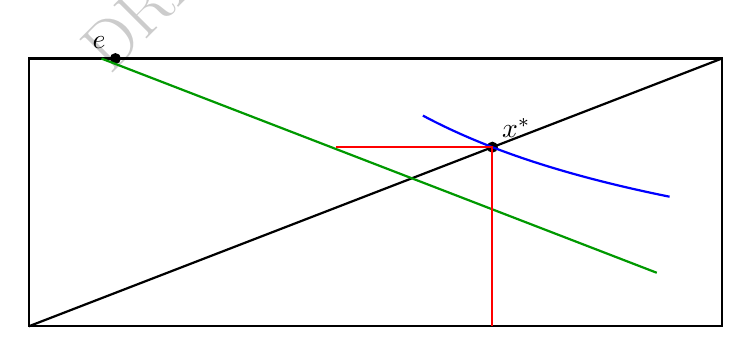
\begin{tikzpicture}[x=1.1cm,y=0.85cm]
  % Box
  \draw[thick] (0,0) rectangle (8,4);

  % Endowment
  \fill (1,4) circle (2pt);
  \node[above left] at (1,4) {$e$};

  % Kink locus
  \draw[black, thick] (0,0) -- (8,4);

  % Competitive equilibrium point
  \coordinate (Xstar) at (5.3523,2.6762);
  \fill (Xstar) circle (2pt);
  \node[above right] at (Xstar) {$x^*$};

  % Budget line through e and x*
  \draw[green!60!black, thick] (0.84,4) -- (7.25,0.80);

  % Astrid indifference curve through x*
  \draw[blue, thick, domain=4.55:7.40, samples=200, smooth]
    plot (\x,{14.3253/\x});

  % Birger indifference curve through x*
  \draw[red, thick] (3.55,2.6762) -- (5.3523,2.6762) -- (5.3523,0);

\end{tikzpicture}
\end{center}

\end{enumerate}

\subsubsection{Method 2: Kink-line geometry and supporting prices}

\begin{enumerate}[label=(\alph*)]
    \item
    The Edgeworth box has total resources
    \[
    (H,C)=(4,8),
    \]
    the endowment is
    \[
    e=(4,1)
    \]
    in Astrid's coordinates, Astrid has smooth Cobb--Douglas indifference curves, and Birger has right-angle indifference curves with kinks where
    \[
    H_B=C_B.
    \]
    In Astrid's coordinates this is
    \[
    \boxed{C_A=H_A+4.}
    \]

    \item
    At a competitive equilibrium Birger chooses a bundle on his kink, so feasible equilibrium allocations must satisfy
    \[
    H_B=C_B.
    \]
    Since
    \[
    H_B=4-H_A,\qquad C_B=8-C_A,
    \]
    this condition becomes
    \[
    4-H_A = 8-C_A
    \qquad\Longrightarrow\qquad
    \boxed{C_A=H_A+4.}
    \]

    Astrid is an interior optimizer because her Cobb--Douglas utility is strictly increasing in both goods. Hence at equilibrium her marginal rate of substitution equals the price ratio:
    \[
    MRS_A=\frac{MU_H}{MU_C}=\frac{C_A}{H_A}=p.
    \]
    Therefore
    \[
    \boxed{C_A=pH_A.}
    \]

    Combining Astrid's tangency with Birger's kink condition,
    \[
    pH_A=H_A+4,
    \]
    so
    \[
    H_A=\frac{4}{p-1}.
    \]
    Then
    \[
    C_A=pH_A=\frac{4p}{p-1}.
    \]

    Astrid must also satisfy her budget constraint. Since the value of her endowment is \(4p+1\),
    \[
    pH_A+C_A=4p+1.
    \]
    Substitute the expressions above:
    \[
    p\left(\frac{4}{p-1}\right)+\frac{4p}{p-1}=4p+1.
    \]
    Thus
    \[
    \frac{8p}{p-1}=4p+1.
    \]
    Multiply by \(p-1\):
    \[
    8p=(4p+1)(p-1)=4p^2-3p-1.
    \]
    Rearranging,
    \[
    4p^2-11p-1=0.
    \]
    Therefore
    \[
    p^{*}=\frac{11+\sqrt{137}}{8}.
    \]

    Now substitute back:
    \[
    H_A^{*}=\frac{4}{p^{*}-1}=\frac{\sqrt{137}-3}{4},
    \]
    \[
    C_A^{*}=p^{*}H_A^{*}=\frac{\sqrt{137}+13}{4}.
    \]
    Hence Birger consumes
    \[
    H_B^{*}=4-H_A^{*}=\frac{19-\sqrt{137}}{4},
    \qquad
    C_B^{*}=8-C_A^{*}=\frac{19-\sqrt{137}}{4}.
    \]

    Therefore
\begin{equation*}
    \boxed{
    \begin{aligned}
        p^{*} &= \frac{11+\sqrt{137}}{8}, \\
        (H_A^{*},C_A^{*}) &= \left(\frac{\sqrt{137}-3}{4},\,\frac{\sqrt{137}+13}{4}\right), \\
        (H_B^{*},C_B^{*}) &= \left(\frac{19-\sqrt{137}}{4},\,\frac{19-\sqrt{137}}{4}\right).
    \end{aligned}
    }
\end{equation*}



    \item
    The competitive equilibrium lies where the price line through the endowment supports Astrid's highest attainable indifference curve and simultaneously passes through a point on Birger's kink line. In Astrid's coordinates that point is
    \[
    \boxed{x^{*}=\left(\frac{\sqrt{137}-3}{4},\,\frac{\sqrt{137}+13}{4}\right).}
    \]
    This is exactly the point marked in the sketch in Method 1.
\end{enumerate}

\newpage
%====================================================
% SAMPLE QUESTION 1
%====================================================
\section{Sample Question 1: Iris and Joseph in a Pure Exchange Economy}

\subsection{Problem}
\begin{itemize}
    \item Consider a small exchange economy, with two consumers Iris and Joseph, and two goods \(X\) and \(Y\). Iris is endowed with 15 units of \(X\) and 3 units of \(Y\). Joseph is endowed with 5 units of \(X\) and 7 units of \(Y\).

    Iris has utility
    \[
    U_I(X,Y)=\min\{X,3Y\}
    \]
    while Joseph has utility
    \[
    U_J(X,Y)=XY.
    \]

    \begin{enumerate}[label=(\alph*)]
        \item Draw the Edgeworth box for this exchange economy as accurately as possible, indicating the endowment and drawing several indifference curves for Iris and Joseph.
        \item In the figure you have drawn in (a), draw the indifference curves through the endowment and indicate where a competitive equilibrium must lie.
        \item Is the allocation where Iris gets \((X=12,Y=4)\) while Joseph gets \((X=8,Y=6)\) a fair allocation? Explain.
        \item ``There always exists an initial endowment for Iris and Joseph where the allocation in the consequent competitive equilibrium is fair for any (standard) preferences of Iris and Joseph.'' True or False? Explain.
    \end{enumerate}
\end{itemize}

\newpage
\subsection{Solution}

\subsubsection{Method 1: Marshallian-demand and market-clearing method}

\begin{enumerate}[label=(\alph*)]
    \item
    Total endowment is
    \[
    (\bar X,\bar Y)=(15+5,\,3+7)=(20,10).
    \]
    Hence the Edgeworth box has width \(20\) and height \(10\).

    Iris has utility
    \[
    U_I(X_I,Y_I)=\min\{X_I,3Y_I\},
    \]
    so her indifference curves are L-shaped, with kinks on the line
    \[
    X_I=3Y_I.
    \]
    Joseph has utility
    \[
    U_J(X_J,Y_J)=X_JY_J,
    \]
    so his indifference curves are smooth, strictly convex hyperbolas drawn from Joseph's origin at the top-right corner.

    The endowment point in Iris coordinates is
    \[
    e=(15,3).
    \]

    Therefore the diagram in part (a) should contain:
    \begin{itemize}
        \item the Edgeworth box \([0,20]\times[0,10]\);
        \item Iris' origin at the bottom-left and Joseph's origin at the top-right;
        \item the endowment point \(e=(15,3)\);
        \item several L-shaped indifference curves for Iris;
        \item several hyperbolic indifference curves for Joseph.
    \end{itemize}

    \item
    Normalise \(P_Y=1\) and write \(P_X=p\).

    Iris' income is
    \[
    m_I=15p+3.
    \]
    Since Iris has perfect-complements preferences, she demands goods in the ratio \(X_I=3Y_I\). Writing \(Y_I=t\), we have \(X_I=3t\), so the budget constraint is
    \[
    3pt+t=15p+3.
    \]
    Hence
    \[
    t=\frac{15p+3}{3p+1},
    \]
    and therefore Iris' demand is
    \[
    X_I=\frac{3(15p+3)}{3p+1},\qquad
    Y_I=\frac{15p+3}{3p+1}.
    \]

    Joseph's income is
    \[
    m_J=5p+7.
    \]
    Since \(U_J(X_J,Y_J)=X_JY_J\) is Cobb--Douglas with equal exponents, Joseph spends half his income on each good:
    \[
    X_J=\frac{m_J}{2p}=\frac{5p+7}{2p},
    \qquad
    Y_J=\frac{m_J}{2}=\frac{5p+7}{2}.
    \]

    Market clearing in good \(Y\) gives
    \[
    \frac{15p+3}{3p+1}+\frac{5p+7}{2}=10.
    \]
    Rearranging,
    \[
    15p^2-4p-7=0.
    \]
    Thus
    \[
    p=\frac{2+\sqrt{109}}{15}>0.
    \]

    So the competitive-equilibrium price ratio is
    \[
    \frac{P_X}{P_Y}=\frac{2+\sqrt{109}}{15}.
    \]

    Substituting into Iris' demand:
    \[
    Y_I^*=\frac{37-\sqrt{109}}{6},
    \qquad
    X_I^*=3Y_I^*=\frac{37-\sqrt{109}}{2}.
    \]
    Hence the competitive equilibrium allocation is
    \[
    x^*=\left(\frac{37-\sqrt{109}}{2},\,\frac{37-\sqrt{109}}{6}\right)
    \approx (13.28,\,4.43)
    \]
    for Iris, and therefore
    \[
    \left(20-\frac{37-\sqrt{109}}{2},\,10-\frac{37-\sqrt{109}}{6}\right)
    =
    \left(\frac{3+\sqrt{109}}{2},\,\frac{23+\sqrt{109}}{6}\right)
    \approx (6.72,\,5.57)
    \]
    for Joseph.

    The indifference curve through the endowment for Iris is
    \[
    U_I(15,3)=\min\{15,9\}=9,
    \]
    so it is the L-shaped indifference curve with kink at
    \[
    (9,3).
    \]
    For Joseph, at the endowment his bundle is \((5,7)\), so
    \[
    U_J(5,7)=35.
    \]
    In Iris coordinates this indifference curve is
    \[
    (20-X_I)(10-Y_I)=35.
    \]

    Since any competitive equilibrium must be Pareto efficient, it must lie on the contract curve. Here the contract curve is the locus of Iris' kink points:
    \[
    X_I=3Y_I.
    \]
    Thus in the diagram for part (b), the competitive equilibrium must lie on this line at the point where a supporting price line through the endowment touches the efficient frontier.

    A suitable Edgeworth box is shown below.

    \begin{center}
    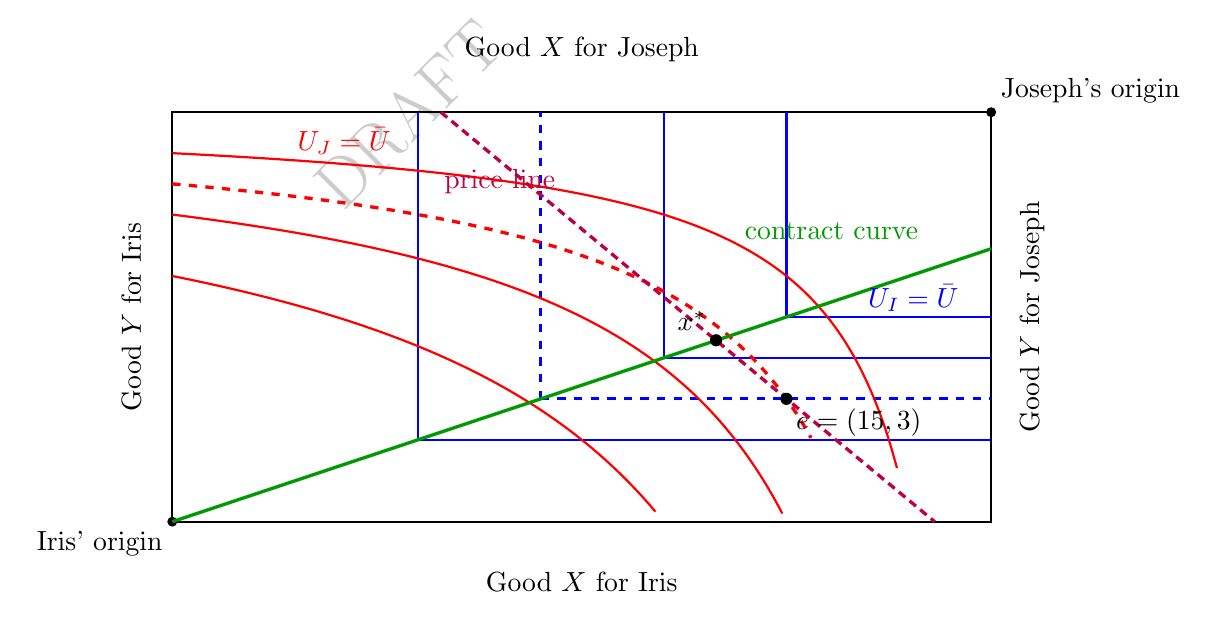
\begin{tikzpicture}[x=0.52cm,y=0.52cm]
      % Edgeworth box
      \draw[thick] (0,0) rectangle (20,10);

      % Origins
      \fill (0,0) circle (1.8pt);
      \fill (20,10) circle (1.8pt);
      \node[below left] at (0,0) {Iris' origin};
      \node[above right] at (20,10) {Joseph's origin};

      % Axis labels
      \node[below] at (10,-1.0) {Good \(X\) for Iris};
      \node[rotate=90] at (-1.0,5) {Good \(Y\) for Iris};
      \node[above] at (10,11.0) {Good \(X\) for Joseph};
      \node[rotate=90] at (21.0,5) {Good \(Y\) for Joseph};

      % Iris indifference curves
      \draw[blue, thick] (6,2) -- (6,10);
      \draw[blue, thick] (6,2) -- (20,2);

      \draw[blue, thick] (12,4) -- (12,10);
      \draw[blue, thick] (12,4) -- (20,4);

      \draw[blue, thick] (15,5) -- (15,10);
      \draw[blue, thick] (15,5) -- (20,5);

      % Iris indifference curve through endowment
      \draw[blue, dashed, very thick] (9,3) -- (9,10);
      \draw[blue, dashed, very thick] (9,3) -- (20,3);

      % Joseph indifference curves
      \draw[red, thick, domain=0:17.7, samples=120, smooth]
        plot (\x,{10-20/(20-\x)});
      \draw[red, thick, domain=0:14.9, samples=120, smooth]
        plot (\x,{10-50/(20-\x)});
      \draw[red, thick, domain=0:11.8, samples=120, smooth]
        plot (\x,{10-80/(20-\x)});

      % Joseph indifference curve through endowment
      \draw[red, dashed, very thick, domain=0:15.6, samples=120, smooth]
        plot (\x,{10-35/(20-\x)});

      % Contract curve
      \draw[green!60!black, very thick] (0,0) -- (20,6.6667);

      % Supporting line through endowment
      \draw[purple, densely dashed, very thick] (6.56,10) -- (18.62,0);

      % Endowment and CE
      \fill (15,3) circle (2.2pt) node[below right] {$e=(15,3)$};
      \fill (13.28,4.43) circle (2.2pt) node[above left] {$x^*$};

      % Labels
      \node[blue] at (18.1,5.45) {$U_I=\bar U$};
      \node[red] at (4.2,9.3) {$U_J=\bar U$};
      \node[green!60!black] at (16.1,7.1) {contract curve};
      \node[purple] at (8.0,8.3) {price line};
    \end{tikzpicture}
    \end{center}

\newpage
    \item
    Under the usual definition of fairness in exchange economies, namely envy-freeness, the proposed allocation is fair if neither consumer prefers the other's bundle to his or her own.

    At the proposed allocation,
    \[
    \text{Iris gets }(12,4),\qquad \text{Joseph gets }(8,6).
    \]

    Iris' utility from her own bundle is
    \[
    U_I(12,4)=\min\{12,12\}=12.
    \]
    If Iris were given Joseph's bundle instead, her utility would be
    \[
    U_I(8,6)=\min\{8,18\}=8.
    \]
    Hence Iris does not envy Joseph.

    Joseph's utility from his own bundle is
    \[
    U_J(8,6)=48.
    \]
    If Joseph were given Iris' bundle instead, his utility would be
    \[
    U_J(12,4)=48.
    \]
    So Joseph is indifferent between the two bundles and therefore does not envy Iris.

    The allocation is also feasible because
    \[
    (12+8,\,4+6)=(20,10).
    \]

    Hence the allocation is envy-free and feasible, so it is fair.

    \item
    The statement is \textbf{True}, under the standard assumptions used for competitive-equilibrium existence.

    A clean argument is to choose the \emph{equal division} of the aggregate endowment as the initial endowment:
    \[
    \omega_I=\omega_J=(10,5).
    \]
    Then both consumers have the same wealth at any given price vector.

    In any competitive equilibrium arising from this equal initial endowment, suppose Iris preferred Joseph's equilibrium bundle to her own. Since both bundles have the same equilibrium value and Iris could afford Joseph's bundle, this would contradict utility maximisation by Iris at equilibrium prices. The same argument applies to Joseph.

    Therefore any competitive equilibrium from an equal division of the aggregate endowment is envy-free, hence fair.

    So for any standard preferences for which a competitive equilibrium exists, there does exist an initial endowment---namely the equal division of the aggregate endowment---such that the consequent competitive equilibrium allocation is fair.
\end{enumerate}

\newpage
\subsubsection{Method 2: Contract-curve parameterisation method}

\begin{enumerate}[label=(\alph*)]
    \item
    Since the total endowment is
    \[
    (20,10),
    \]
    the Edgeworth box is again \([0,20]\times[0,10]\).

    Iris has Leontief-type preferences
    \[
    U_I(X_I,Y_I)=\min\{X_I,3Y_I\},
    \]
    so her indifference curves are L-shaped with kinks on
    \[
    X_I=3Y_I.
    \]
    Joseph's indifference curves are hyperbolas from the opposite origin because
    \[
    U_J(X_J,Y_J)=X_JY_J.
    \]
    The endowment point is
    \[
    e=(15,3).
    \]

    \item
    The key observation is that at any efficient allocation Iris must be at a kink:
    \[
    X_I=3Y_I.
    \]
    Hence efficient candidate allocations can be parameterised as
    \[
    (X_I,Y_I)=(3t,t),
    \qquad 0\le t\le \frac{20}{3}.
    \]
    Then Joseph receives
    \[
    (X_J,Y_J)=(20-3t,\,10-t).
    \]

    At a smooth point of Joseph's indifference curve, the supporting price ratio must satisfy
    \[
    \frac{P_X}{P_Y}=MRS_J=\frac{MU_X}{MU_Y}
    =\frac{Y_J}{X_J}
    =\frac{10-t}{20-3t}.
    \]
    Writing \(P_Y=1\) and \(P_X=p\), we therefore have
    \[
    p=\frac{10-t}{20-3t}.
    \]

    Since the equilibrium allocation must lie on the budget line through the endowment \(e=(15,3)\), Iris' bundle \((3t,t)\) must satisfy
    \[
    3pt+t=15p+3.
    \]
    Substituting
    \[
    p=\frac{10-t}{20-3t}
    \]
    into this equation yields
    \[
    3t^2-37t+105=0.
    \]
    Hence
    \[
    t=\frac{37\pm \sqrt{109}}{6}.
    \]
    The larger root is infeasible because it would imply \(3t>20\). Thus
    \[
    t=\frac{37-\sqrt{109}}{6}.
    \]

    Therefore the competitive equilibrium allocation is
    \[
    (X_I^*,Y_I^*)=(3t,t)
    =
    \left(\frac{37-\sqrt{109}}{2},\,\frac{37-\sqrt{109}}{6}\right),
    \]
    which is the same point found in Method 1.

    The indifference curves through the endowment are:
    \[
    U_I(15,3)=9
    \quad\Longrightarrow\quad
    \text{Iris' endowment indifference curve has kink at }(9,3),
    \]
    and
    \[
    U_J(5,7)=35
    \quad\Longrightarrow\quad
    (20-X_I)(10-Y_I)=35
    \]
    for Joseph in Iris coordinates.

    Thus the competitive equilibrium must lie on the contract curve
    \[
    X_I=3Y_I
    \]
    at the point where the supporting price line through the endowment touches the efficient set.

    \item
    At the proposed allocation
    \[
    \text{Iris gets }(12,4),\qquad \text{Joseph gets }(8,6),
    \]
    Iris' utility is
    \[
    U_I(12,4)=\min\{12,12\}=12,
    \]
    while if she were given Joseph's bundle, her utility would be
    \[
    U_I(8,6)=\min\{8,18\}=8.
    \]
    So Iris strictly prefers her own bundle.

    Joseph's utility from his own bundle is
    \[
    U_J(8,6)=48,
    \]
    and from Iris' bundle it is
    \[
    U_J(12,4)=48.
    \]
    Thus Joseph is indifferent.

    Since the allocation is feasible and neither person envies the other, it is fair.

    \item
    The statement is \textbf{True}.

    The structural reason is that one may choose the initial endowment to be the equal division of total resources:
    \[
    \omega_I=\omega_J=(10,5).
    \]
    Then both consumers enter the market with equal wealth. In any competitive equilibrium from such an equal division, each agent's chosen equilibrium bundle is at least as good as any other affordable bundle. Since the other consumer's bundle has exactly the same value at equilibrium prices, neither agent can prefer the other's bundle.

    Hence the resulting competitive equilibrium is envy-free, and therefore fair.
\end{enumerate}

\newpage
\subsubsection{Method 3: Supporting-prices and envy-freeness theorem method}

\begin{enumerate}[label=(\alph*)]
    \item
    The Edgeworth box is determined by aggregate resources
    \[
    (\bar X,\bar Y)=(20,10).
    \]
    Iris' preferences generate right-angled indifference curves with corners on
    \[
    X_I=3Y_I,
    \]
    while Joseph's preferences generate smooth hyperbolas from Joseph's origin.

    The endowment is
    \[
    e=(15,3)
    \]
    in Iris coordinates.

    \item
    A competitive equilibrium must be both feasible and Pareto efficient. Since Iris only values bundles through the smaller of \(X_I\) and \(3Y_I\), any efficient allocation must place her at a kink, hence on
    \[
    X_I=3Y_I.
    \]
    So even before calculation, one knows that the competitive equilibrium must lie on this line.

    To recover the exact equilibrium, normalise \(P_Y=1\) and let \(P_X=p\). At any competitive equilibrium, Joseph's smooth indifference curve must be tangent to the common supporting price line, so
    \[
    p=\frac{Y_J}{X_J}.
    \]
    Using feasibility with
    \[
    (X_I,Y_I)=(3t,t)
    \quad\text{and}\quad
    (X_J,Y_J)=(20-3t,10-t),
    \]
    this gives
    \[
    p=\frac{10-t}{20-3t}.
    \]
    Since Iris' chosen bundle must lie on the budget line through the endowment,
    \[
    3pt+t=15p+3.
    \]
    Solving yields
    \[
    t=\frac{37-\sqrt{109}}{6},
    \]
    so
    \[
    x^*=
    \left(\frac{37-\sqrt{109}}{2},\,\frac{37-\sqrt{109}}{6}\right).
    \]

    The indifference curves through the endowment are obtained from
    \[
    U_I(15,3)=9
    \quad\text{and}\quad
    U_J(5,7)=35.
    \]
    Hence Iris' endowment indifference curve has kink at \((9,3)\), while Joseph's is
    \[
    (20-X_I)(10-Y_I)=35.
    \]

    \item
    Fairness is checked by envy-freeness.

    For Iris:
    \[
    U_I(12,4)=12,
    \qquad
    U_I(8,6)=8.
    \]
    So Iris does not envy Joseph.

    For Joseph:
    \[
    U_J(8,6)=48,
    \qquad
    U_J(12,4)=48.
    \]
    So Joseph is indifferent and does not envy Iris.

    Therefore the allocation is fair.

    \item
    The statement is \textbf{True}. A standard theorem states that a competitive equilibrium with equal incomes is envy-free. Therefore, if one chooses the initial endowment to split the aggregate resources equally between the two consumers, any competitive equilibrium that results is fair.

    In this economy the equal split is
    \[
    \omega_I=\omega_J=(10,5).
    \]
    Thus there always exists an initial endowment that yields a fair competitive equilibrium.
\end{enumerate}
\vspace{3cm}
\subsubsection{Marking scheme (30 marks)}

\begin{enumerate}[label=(\alph*)]
    \item \textbf{(6 marks)} Edgeworth box and indifference curves
    \begin{itemize}
        \item 1 mark: Correct total endowment and hence correct dimensions of the Edgeworth box, namely \((20,10)\).
        \item 1 mark: Correct placement of Iris' and Joseph's origins, together with the correct endowment point \(e=(15,3)\) in Iris coordinates.
        \item 2 marks: Correct depiction of Iris' indifference curves as L-shaped, with kinks on the line \(X_I=3Y_I\).
        \item 2 marks: Correct depiction of Joseph's indifference curves as smooth convex hyperbolas from Joseph's origin.
    \end{itemize}

\newpage
    \item \textbf{(10 marks)} Indifference curves through the endowment and competitive equilibrium location
    \begin{itemize}
        \item 2 marks: Correct utility level for Iris at the endowment and hence correct indifference curve through the endowment, namely \(U_I(15,3)=9\) with kink at \((9,3)\).
        \item 2 marks: Correct utility level for Joseph at the endowment and hence correct indifference curve through the endowment, namely \(U_J(5,7)=35\), or an equivalent correctly drawn curve.
        \item 2 marks: Correct identification that any competitive equilibrium must be Pareto efficient and therefore lie on the contract curve.
        \item 2 marks: Correct identification of the contract curve / efficient locus as \(X_I=3Y_I\), i.e. Iris must be at a kink.
        \item 2 marks: Correct indication of a supporting price line through the endowment and a correct equilibrium location on the contract curve; full credit also if the exact competitive-equilibrium allocation is correctly computed.
    \end{itemize}

    \item \textbf{(6 marks)} Fairness of the allocation \((12,4)\) for Iris and \((8,6)\) for Joseph
    \begin{itemize}
        \item 2 marks: Correct computation of Iris' utility from her own bundle and from Joseph's bundle, with the correct conclusion that Iris does not envy Joseph.
        \item 2 marks: Correct computation of Joseph's utility from his own bundle and from Iris' bundle, with the correct conclusion that Joseph is indifferent and hence does not envy Iris.
        \item 1 mark: Correct verification of feasibility.
        \item 1 mark: Correct final conclusion that the allocation is fair under the envy-free interpretation.
    \end{itemize}

    \item \textbf{(8 marks)} Existence of an initial endowment yielding a fair competitive equilibrium
    \begin{itemize}
        \item 2 marks: Correct statement that the claim is \textbf{True}.
        \item 3 marks: Correct construction or explanation using equal division of the aggregate endowment, or an equivalent equal-income argument.
        \item 2 marks: Correct use of the competitive-equilibrium / equal-income intuition that each consumer weakly prefers his or her own equilibrium bundle to the other's bundle, so the equilibrium is envy-free.
        \item 1 mark: Clear final conclusion that there always exists such an initial endowment under standard assumptions.
    \end{itemize}
\end{enumerate}
%====================================================
% SAMPLE QUESTION 2
%====================================================
\newpage
\section{Sample Question 2: Leontief and Cobb--Douglas in a Pure Exchange Economy}

\subsection{Problem}
\begin{itemize}
    \item Consider the following two-good, two-person exchange economy.

    Person A has an endowment of 5 units of good \(X\) and 10 units of good \(Y\). He has preferences
    \[
    U_A(X,Y)=\min(X,Y).
    \]

    Person B has an endowment of 10 units of good \(X\) and 5 units of good \(Y\). He has preferences
    \[
    U_B(X,Y)=X^{0.4}Y^{0.6}.
    \]

    \begin{enumerate}[label=(\alph*)]
        \item Calculate the competitive equilibrium prices and allocations. You can assume that \(P_Y=1\).
        \item In an Edgeworth Box with Person A at the bottom left, Person B on the top right, good \(X\) on the \(x\)-axis and good \(Y\) on the \(y\)-axis, indicate the endowment and illustrate the competitive equilibrium of this economy.
    \end{enumerate}

    Let \((a,b)\) denote the feasible allocation where Person A receives \(a\) units of good \(X\) and \(b\) units of good \(Y\). This implies that Person B receives \(15-a\) units of good \(X\) and \(15-b\) units of good \(Y\).

    \begin{enumerate}[label=(\alph*),resume]
        \item Consider the feasible allocation \((7,7)\). Show that this is Pareto efficient and provide an endowment different from \((7,7)\) which will result in it being a competitive equilibrium after trading.
        \item ``For any exchange economy, the competitive equilibrium after trading will also be fair.'' True or False? Explain.
    \end{enumerate}
\end{itemize}

\newpage
\subsection{Solution}

\subsubsection{Method 1: Marshallian-demand and market-clearing method}

\begin{enumerate}[label=(\alph*)]
    \item
    Total endowment is
    \[
    (\bar X,\bar Y)=(5+10,\,10+5)=(15,15).
    \]

    Normalise \(P_Y=1\) and write \(P_X=p\).

    Person A has income
    \[
    m_A=5p+10.
    \]
    Since
    \[
    U_A(X,Y)=\min(X,Y),
    \]
    A chooses equal quantities of the two goods:
    \[
    X_A=Y_A=t.
    \]
    Using the budget constraint,
    \[
    pt+t=m_A=5p+10,
    \]
    so
    \[
    t=\frac{5p+10}{p+1}.
    \]
    Therefore
    \[
    X_A=Y_A=\frac{5p+10}{p+1}.
    \]

    Person B has income
    \[
    m_B=10p+5.
    \]
    Since B has Cobb--Douglas utility \(X^{0.4}Y^{0.6}\), the Marshallian demands are
    \[
    X_B=0.4\frac{m_B}{p},
    \qquad
    Y_B=0.6m_B.
    \]
    Hence
    \[
    X_B=0.4\frac{10p+5}{p},
    \qquad
    Y_B=0.6(10p+5).
    \]

    Market clearing in good \(X\) gives
    \[
    \frac{5p+10}{p+1}+0.4\frac{10p+5}{p}=15.
    \]
    Simplifying,
    \[
    \frac{5p+10}{p+1}+4+\frac{2}{p}=15,
    \]
    so
    \[
    \frac{5p+10}{p+1}+\frac{2}{p}=11.
    \]
    Multiply through by \(p(p+1)\):
    \[
    p(5p+10)+2(p+1)=11p(p+1).
    \]
    Therefore
    \[
    5p^2+10p+2p+2=11p^2+11p,
    \]
    hence
    \[
    6p^2-p-2=0.
    \]
    So
    \[
    p=\frac{1\pm 7}{12}.
    \]
    Since price must be positive,
    \[
    p=\frac23.
    \]

    Therefore the competitive-equilibrium prices are
    \[
    (P_X,P_Y)=\left(\frac23,1\right).
    \]

    Substituting back,
    \[
    m_A=5\cdot\frac23+10=\frac{40}{3},
    \]
    so
    \[
    X_A=Y_A=\frac{40/3}{5/3}=8.
    \]
    Thus
    \[
    (X_A,Y_A)=(8,8).
    \]

    Similarly,
    \[
    m_B=10\cdot\frac23+5=\frac{35}{3},
    \]
    and
    \[
    X_B=0.4\cdot\frac{35/3}{2/3}=7,
    \qquad
    Y_B=0.6\cdot\frac{35}{3}=7.
    \]
    Hence
    \[
    (X_B,Y_B)=(7,7).
    \]

    So the competitive equilibrium allocation is
    \[
    A:(8,8),\qquad B:(7,7).
    \]
\newpage
    \item
    The Edgeworth box has width \(15\) and height \(15\). The endowment point is
    \[
    e=(5,10)
    \]
    in A-coordinates, and the competitive equilibrium is
    \[
    x^*=(8,8)
    \]
    for A, equivalently \((7,7)\) for B.

    A's indifference curves are L-shaped with kinks on
    \[
    X_A=Y_A,
    \]
    while B's indifference curves are smooth and convex from B's origin at the top-right.

    A suitable Edgeworth box is shown below.

    \begin{center}
    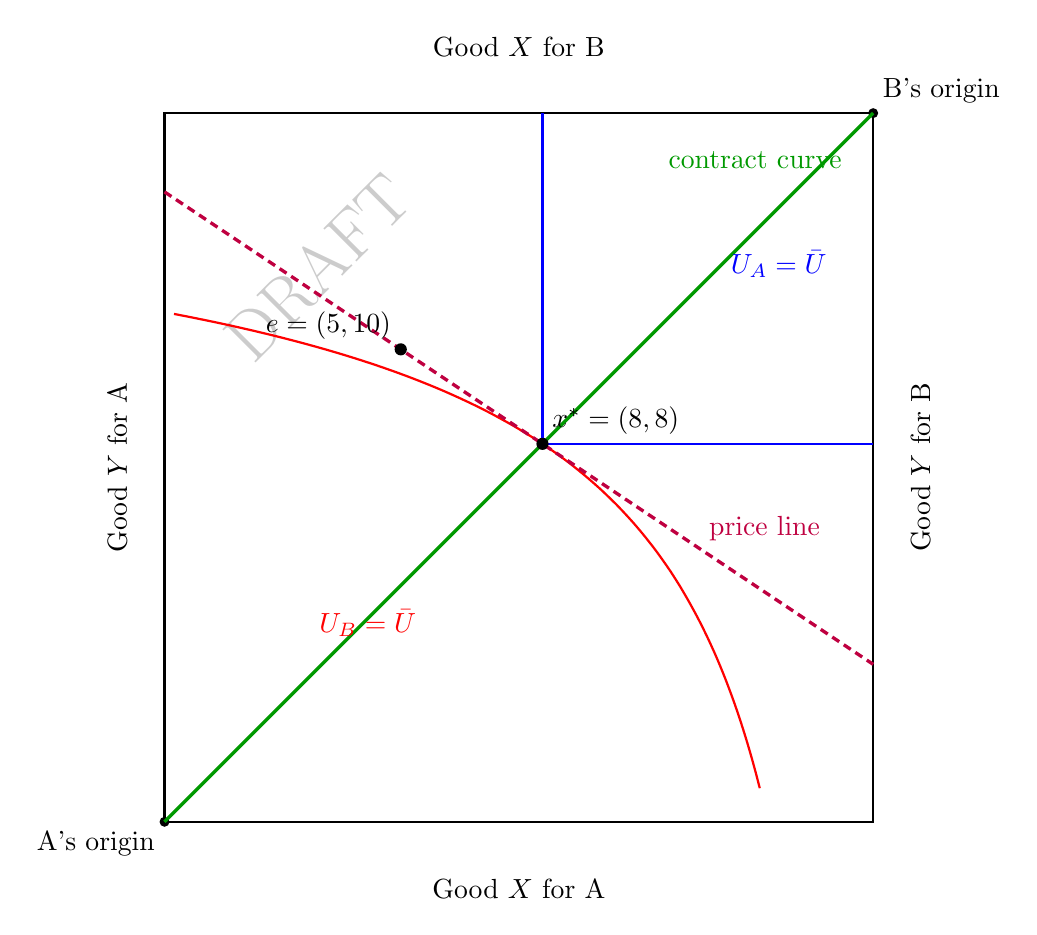
\begin{tikzpicture}[x=0.60cm,y=0.60cm]
      % Edgeworth box
      \draw[thick] (0,0) rectangle (15,15);

      % Origins
      \fill (0,0) circle (1.8pt);
      \fill (15,15) circle (1.8pt);
      \node[below left] at (0,0) {A's origin};
      \node[above right] at (15,15) {B's origin};

      % Axis labels
      \node[below] at (7.5,-1.0) {Good \(X\) for A};
      \node[rotate=90] at (-1.0,7.5) {Good \(Y\) for A};
      \node[above] at (7.5,16.0) {Good \(X\) for B};
      \node[rotate=90] at (16.0,7.5) {Good \(Y\) for B};

      % A indifference curve
      \draw[blue, thick] (8,8) -- (8,15);
      \draw[blue, thick] (8,8) -- (15,8);

      % B indifference curve through equilibrium
      \draw[red, thick, domain=0.2:12.6, samples=140, smooth]
        plot (\x,{15-((7)/((15-\x)^0.4))^(1/0.6)});

      % Contract curve
      \draw[green!60!black, very thick] (0,0) -- (15,15);

      % Budget line
      \draw[purple, densely dashed, very thick] (0,13.333) -- (15,3.333);

      % Endowment and equilibrium
      \fill (5,10) circle (2.2pt) node[above left] {$e=(5,10)$};
      \fill (8,8) circle (2.2pt) node[above right] {$x^*=(8,8)$};

      % Labels
      \node[blue] at (13.0,11.8) {$U_A=\bar U$};
      \node[red] at (4.3,4.2) {$U_B=\bar U$};
      \node[green!60!black] at (12.5,14.0) {contract curve};
      \node[purple] at (12.7,6.2) {price line};
    \end{tikzpicture}
    \end{center}

\newpage
    \item
    At the feasible allocation \((7,7)\), A receives
    \[
    (7,7)
    \]
    and B receives
    \[
    (8,8).
    \]

    To show Pareto efficiency, use supporting prices. At B's bundle \((8,8)\),
    \[
    MRS_B=\frac{MU_X}{MU_Y}
    =\frac{0.4X_B^{-0.6}Y_B^{0.6}}{0.6X_B^{0.4}Y_B^{-0.4}}
    =\frac{0.4}{0.6}\frac{Y_B}{X_B}
    =\frac23.
    \]
    So the supporting price ratio is
    \[
    \frac{P_X}{P_Y}=\frac23.
    \]

    At A's bundle \((7,7)\), A is exactly at the kink of the Leontief indifference curve \(X_A=Y_A\), so this same price ratio can support A's optimum. Therefore there exists a common supporting price vector, and hence \((7,7)\) is Pareto efficient.

    To produce \((7,7)\) as a competitive equilibrium after trade, choose an initial endowment for A that is different from \((7,7)\) but lies on the same budget line through \((7,7)\) at prices \(\left(\frac23,1\right)\). For example, take
    \[
    \omega_A'=(4,9).
    \]
    Then B's endowment is
    \[
    \omega_B'=(11,6).
    \]
    Check the value of A's endowment:
    \[
    \frac23\cdot 4+9=\frac{35}{3}.
    \]
    The value of A's target bundle \((7,7)\) is
    \[
    \frac23\cdot 7+7=\frac{35}{3}.
    \]
    So A can afford \((7,7)\), and similarly B can afford \((8,8)\). Hence with the endowment profile
    \[
    \omega_A'=(4,9),\qquad \omega_B'=(11,6),
    \]
    the allocation
    \[
    A:(7,7),\qquad B:(8,8)
    \]
    is a competitive equilibrium after trading.
\newpage
    \item
    The statement is \textbf{False}.

    Competitive equilibrium guarantees Pareto efficiency under standard assumptions, but it does \emph{not} guarantee fairness or envy-freeness for arbitrary initial endowments.

    A concrete counterexample can be built in this very economy. Suppose A initially owns everything:
    \[
    \omega_A=(15,15),\qquad \omega_B=(0,0).
    \]
    Take prices
    \[
    (P_X,P_Y)=(1,1).
    \]
    Then A's income is \(30\), and since A has utility \(\min(X,Y)\), A chooses
    \[
    (15,15).
    \]
    B has zero income and therefore chooses
    \[
    (0,0).
    \]
    Thus no trade is a competitive equilibrium.

    But this allocation is not fair, because B strictly prefers A's bundle:
    \[
    U_B(15,15)>U_B(0,0).
    \]
    Hence competitive equilibrium need not be fair.
\end{enumerate}

\newpage
\subsubsection{Method 2: Contract-curve and supporting-price method}

\begin{enumerate}[label=(\alph*)]
    \item
    Since
    \[
    U_A(X,Y)=\min(X,Y),
    \]
    any efficient allocation must put A at a kink:
    \[
    X_A=Y_A.
    \]
    So write
    \[
    (X_A,Y_A)=(t,t).
    \]
    By feasibility, B then receives
    \[
    (X_B,Y_B)=(15-t,15-t).
    \]

    At B's bundle, the Cobb--Douglas marginal rate of substitution is
    \[
    MRS_B=\frac{0.4}{0.6}\frac{Y_B}{X_B}
    =\frac{0.4}{0.6}\cdot 1
    =\frac23.
    \]
    Hence any interior supporting price vector must satisfy
    \[
    \frac{P_X}{P_Y}=\frac23.
    \]
    Normalising \(P_Y=1\), we get
    \[
    P_X=\frac23.
    \]

    A's income at the initial endowment \((5,10)\) is
    \[
    m_A=5\cdot\frac23+10=\frac{40}{3}.
    \]
    Since A chooses equal quantities,
    \[
    \frac23 t+t=\frac{40}{3}.
    \]
    Hence
    \[
    \frac53 t=\frac{40}{3}
    \quad\Longrightarrow\quad
    t=8.
    \]

    Therefore the competitive equilibrium allocation is
    \[
    A:(8,8),\qquad B:(7,7),
    \]
    with prices
    \[
    \left(\frac23,1\right).
    \]

    \item
    In the Edgeworth box, the endowment is
    \[
    e=(5,10),
    \]
    and the equilibrium is
    \[
    x^*=(8,8).
    \]
    The contract curve is the diagonal
    \[
    X_A=Y_A,
    \]
    because A must be at a kink at any efficient allocation and total resources of the two goods are equal.

    Hence the correct diagram has:
    \begin{itemize}
        \item the \(15\times 15\) Edgeworth box;
        \item A's origin at the bottom-left and B's origin at the top-right;
        \item the endowment \(e=(5,10)\);
        \item the equilibrium point \(x^*=(8,8)\);
        \item A's L-shaped indifference curve through \((8,8)\);
        \item B's smooth indifference curve through \((7,7)\) from B's origin;
        \item a supporting price line of slope \(-\frac23\) through the endowment and equilibrium.
    \end{itemize}

    \item
    For the allocation \((7,7)\), A gets \((7,7)\) and B gets \((8,8)\).

    A is exactly at a Leontief kink. At B's bundle,
    \[
    MRS_B=\frac23.
    \]
    Hence the price ratio
    \[
    \frac{P_X}{P_Y}=\frac23
    \]
    supports B's optimum and is also consistent with A being at a kink. Therefore \((7,7)\) is Pareto efficient.

    To make \((7,7)\) arise as a competitive equilibrium after trade, pick any different endowment for A on the same budget line through \((7,7)\). For instance,
    \[
    \omega_A'=(4,9),
    \qquad
    \omega_B'=(11,6).
    \]
    At prices \(\left(\frac23,1\right)\), \((7,7)\) has the same value as \((4,9)\), so the target allocation is supported.

    \item
    The statement is \textbf{False}. Efficiency does not imply fairness.

    In this same economy, if A owns all resources initially,
    \[
    \omega_A=(15,15),\qquad \omega_B=(0,0),
    \]
    then a no-trade competitive equilibrium exists, but B envies A. So a competitive equilibrium need not be fair.
\end{enumerate}

\newpage
\subsubsection{Method 3: Expenditure-share and counterexample method}

\begin{enumerate}[label=(\alph*)]
    \item
    Let \(P_Y=1\) and \(P_X=p\).

    A always chooses equal quantities because
    \[
    U_A(X,Y)=\min(X,Y).
    \]
    Hence A's demand must take the form
    \[
    (X_A,Y_A)=(t,t).
    \]
    Since A's income is \(5p+10\), this gives
    \[
    pt+t=5p+10
    \quad\Longrightarrow\quad
    t=\frac{5p+10}{p+1}.
    \]

    B has Cobb--Douglas utility \(X^{0.4}Y^{0.6}\), so B spends \(40\%\) of income on \(X\) and \(60\%\) on \(Y\). Therefore,
    \[
    X_B=0.4\frac{10p+5}{p},
    \qquad
    Y_B=0.6(10p+5).
    \]

    Using one market-clearing equation,
    \[
    \frac{5p+10}{p+1}+0.4\frac{10p+5}{p}=15,
    \]
    which simplifies to
    \[
    6p^2-p-2=0.
    \]
    Hence
    \[
    p=\frac23.
    \]
    Substituting gives
    \[
    A:(8,8),\qquad B:(7,7).
    \]

    \item
    The Edgeworth-box picture is then immediate:
    \begin{itemize}
        \item total resources are \((15,15)\), so the box is \(15\times 15\);
        \item the endowment is \(e=(5,10)\);
        \item the competitive equilibrium is \(x^*=(8,8)\) for A;
        \item the price line has slope \(-\frac23\);
        \item the equilibrium lies on the diagonal \(X_A=Y_A\), which is the efficient locus generated by A's Leontief preferences.
    \end{itemize}
\newpage
    \item
    At allocation \((7,7)\), A's bundle is exactly balanced, so A is at a kink. B receives \((8,8)\), and at that bundle
    \[
    MRS_B=\frac{0.4}{0.6}\frac{8}{8}=\frac23.
    \]
    Therefore a supporting price line with slope \(-\frac23\) exists, so the allocation is Pareto efficient.

    A different endowment that supports this allocation is
    \[
    \omega_A'=(4,9),
    \qquad
    \omega_B'=(11,6).
    \]
    At prices \(\left(\frac23,1\right)\), both consumers can afford their target bundles, and these bundles are utility-maximising, so the target allocation is a competitive equilibrium after trade.

    \item
    The statement is \textbf{False}. A competitive equilibrium can be efficient but highly unequal.

    For example, if
    \[
    \omega_A=(15,15),\qquad \omega_B=(0,0),
    \]
    then no trade can be a competitive equilibrium, yet B envies A. Therefore competitive equilibrium after trade need not be fair in general.
\end{enumerate}

\newpage
\subsubsection{Marking scheme (30 marks)}

\begin{enumerate}[label=(\alph*)]
    \item \textbf{(10 marks)} Competitive equilibrium prices and allocations
    \begin{itemize}
        \item 2 marks: Correct incomes for A and B after normalising \(P_Y=1\) and writing \(P_X=p\).
        \item 2 marks: Correct demand for A using the Leontief structure \(X_A=Y_A\).
        \item 2 marks: Correct Marshallian demand for B using the Cobb--Douglas expenditure shares.
        \item 2 marks: Correct market-clearing equation and correct equilibrium price \(p=\frac23\).
        \item 2 marks: Correct equilibrium allocations \(A:(8,8)\) and \(B:(7,7)\).
    \end{itemize}

    \item \textbf{(6 marks)} Edgeworth-box illustration of the equilibrium
    \begin{itemize}
        \item 1 mark: Correct dimensions of the Edgeworth box, namely \((15,15)\).
        \item 1 mark: Correct endowment point \(e=(5,10)\) in A-coordinates.
        \item 1 mark: Correct equilibrium point \(x^*=(8,8)\) in A-coordinates.
        \item 1 mark: Correct depiction of A's indifference curves as L-shaped with kinks on \(X_A=Y_A\).
        \item 1 mark: Correct depiction of B's indifference curves as smooth convex curves from B's origin.
        \item 1 mark: Correct indication of the supporting price line and / or the contract curve through the equilibrium.
    \end{itemize}

    \item \textbf{(8 marks)} Pareto efficiency of \((7,7)\) and supporting endowment
    \begin{itemize}
        \item 2 marks: Correct identification of the implied bundle for B, namely \((8,8)\).
        \item 2 marks: Correct supporting-price or marginal-rate-of-substitution argument showing that \((7,7)\) is Pareto efficient.
        \item 2 marks: Correct construction of an endowment different from \((7,7)\) that lies on the supporting budget line through the target allocation, for example \((4,9)\) for A.
        \item 2 marks: Correct verification that the proposed endowment supports \((7,7)\) as a competitive equilibrium after trade, or an equivalent correct supporting argument.
    \end{itemize}

    \item \textbf{(6 marks)} Fairness of competitive equilibrium in general
    \begin{itemize}
        \item 2 marks: Correct statement that the claim is \textbf{False}.
        \item 2 marks: Correct explanation that competitive equilibrium guarantees Pareto efficiency, not fairness or envy-freeness in general.
        \item 2 marks: Correct counterexample or equivalent reasoning showing that a competitive equilibrium can be efficient but not fair.
    \end{itemize}
\end{enumerate}

\end{document}
% Add this to your preamble if not already included:
% \usepackage{tikz}

\newpage
\section{Question 1}
\subsubsection{Solution}

Let Iris's allocation be \((x_I,y_I)\). Since the aggregate endowment is
\[
(15+5,\;3+7)=(20,10),
\]
Joseph's allocation is
\[
(x_J,y_J)=(20-x_I,\;10-y_I).
\]

\begin{enumerate}[label=(\alph*)]
    \item
    The Edgeworth box has width \(20\) and height \(10\).

    Iris's initial endowment is
    \[
    \omega_I=(15,3),
    \]
    so the endowment point in Iris's coordinates is
    \[
    \omega=(15,3).
    \]
    Equivalently, from Joseph's origin at the top right, the endowment is
    \[
    \omega_J=(5,7).
    \]

    Iris has utility
    \[
    U_I(x_I,y_I)=\min\{x_I,3y_I\}.
    \]
    Hence her indifference curve for utility level \(\bar u\) is L-shaped with kink at
    \[
    \left(\bar u,\frac{\bar u}{3}\right),
    \]
    so the kink locus is
    \[
    x_I=3y_I.
    \]

    Joseph has utility
    \[
    U_J(x_J,y_J)=x_Jy_J.
    \]
    In Iris's coordinates this becomes
    \[
    U_J=(20-x_I)(10-y_I),
    \]
    so Joseph's indifference curves are rectangular hyperbolas relative to Joseph's origin.

    A suitable Edgeworth box is shown below. The dashed blue and dashed red curves are the indifference curves through the endowment, which will be used again in part (b).

    \begin{center}
    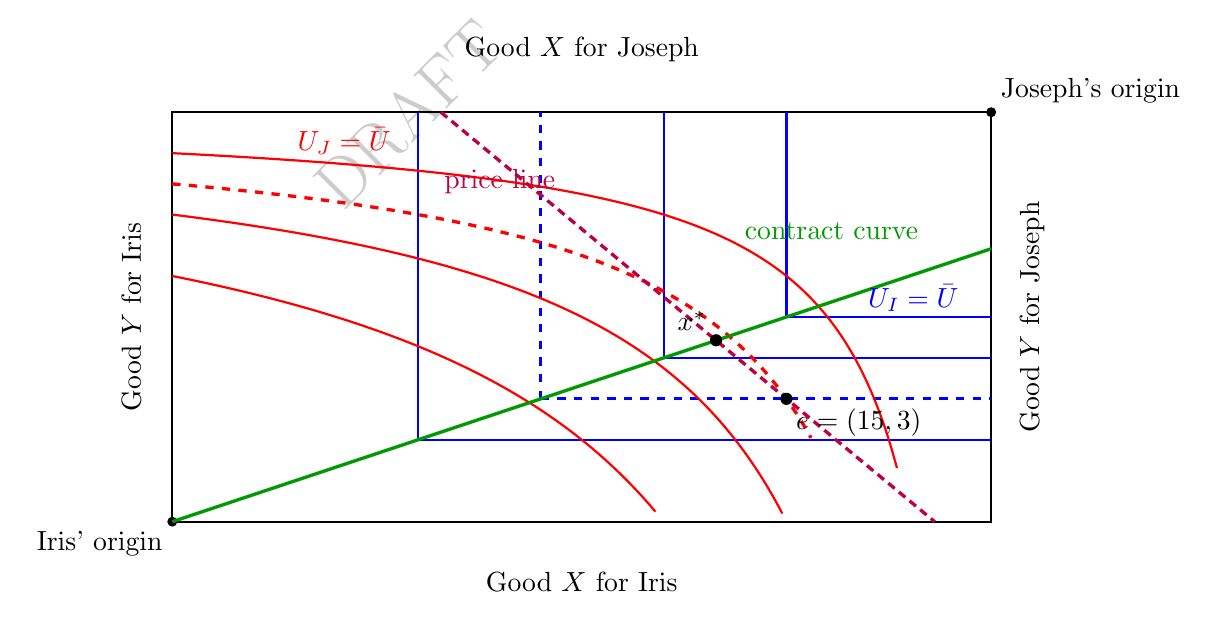
\begin{tikzpicture}[x=0.52cm,y=0.52cm]
      % Edgeworth box
      \draw[thick] (0,0) rectangle (20,10);

      % Origins
      \fill (0,0) circle (1.8pt);
      \fill (20,10) circle (1.8pt);
      \node[below left] at (0,0) {Iris' origin};
      \node[above right] at (20,10) {Joseph's origin};

      % Axis labels
      \node[below] at (10,-1.0) {Good \(X\) for Iris};
      \node[rotate=90] at (-1.0,5) {Good \(Y\) for Iris};
      \node[above] at (10,11.0) {Good \(X\) for Joseph};
      \node[rotate=90] at (21.0,5) {Good \(Y\) for Joseph};

      % Iris indifference curves (solid blue)
      \draw[blue, thick] (6,2) -- (6,10);
      \draw[blue, thick] (6,2) -- (20,2);

      \draw[blue, thick] (12,4) -- (12,10);
      \draw[blue, thick] (12,4) -- (20,4);

      \draw[blue, thick] (15,5) -- (15,10);
      \draw[blue, thick] (15,5) -- (20,5);

      % Iris indifference curve through endowment: u=9
      \draw[blue, dashed, very thick] (9,3) -- (9,10);
      \draw[blue, dashed, very thick] (9,3) -- (20,3);

      % Joseph indifference curves (solid red): (20-x)(10-y)=k
      \draw[red, thick, domain=0:17.7, samples=120, smooth]
        plot (\x,{10-20/(20-\x)});
      \draw[red, thick, domain=0:14.9, samples=120, smooth]
        plot (\x,{10-50/(20-\x)});
      \draw[red, thick, domain=0:11.8, samples=120, smooth]
        plot (\x,{10-80/(20-\x)});

      % Joseph indifference curve through endowment: k=35
      \draw[red, dashed, very thick, domain=0:15.6, samples=120, smooth]
        plot (\x,{10-35/(20-\x)});

      % Contract curve x = 3y  -> y = x/3
      \draw[green!60!black, very thick] (0,0) -- (20,6.6667);

      % Competitive budget/supporting line through endowment and CE
      \draw[purple, densely dashed, very thick] (6.56,10) -- (18.62,0);

      % Endowment and CE
      \fill (15,3) circle (2.2pt) node[below right] {$e=(15,3)$};
      \fill (13.28,4.43) circle (2.2pt) node[above left] {$x^*$};

      % Labels
      \node[blue] at (18.1,5.45) {$U_I=\bar U$};
      \node[red] at (4.2,9.3) {$U_J=\bar U$};
      \node[green!60!black] at (16.1,7.1) {contract curve};
      \node[purple] at (8.0,8.3) {price line};
    \end{tikzpicture}
    \end{center}

    \item
    First compute the utilities at the endowment:
    \[
    U_I(\omega)=\min\{15,3\cdot 3\}=\min\{15,9\}=9,
    \]
    \[
    U_J(\omega)=5\cdot 7=35.
    \]

    So the indifference curves through the endowment are:
    \[
    \min\{x_I,3y_I\}=9
    \]
    for Iris, and
    \[
    (20-x_I)(10-y_I)=35
    \]
    for Joseph.

    Any competitive equilibrium must satisfy two properties:

    \textbf{(i) Individual rationality:} each consumer must be weakly better off than at the endowment, so
    \[
    \min\{x_I,3y_I\}\ge 9,
    \qquad
    (20-x_I)(10-y_I)\ge 35.
    \]

    \textbf{(ii) Pareto efficiency:} the allocation must lie on the contract curve.

    For this economy, the contract curve is
    \[
    \boxed{x_I=3y_I.}
    \]
    The reason is that if \(x_I>3y_I\), Iris has excess \(X\) that does not raise her utility, while if \(x_I<3y_I\), she has excess \(Y\) that does not raise her utility. In either case, some of that excess can be transferred to Joseph without hurting Iris, so such allocations are not Pareto efficient.

    Therefore the competitive equilibrium must lie on the part of the line \(x_I=3y_I\) that is inside the lens formed by the two indifference curves through the endowment, as indicated in the diagram above.

    To find the exact competitive equilibrium, normalize \(p_Y=1\) and let \(p_X=p\).

    Iris's wealth is
    \[
    m_I=15p+3.
    \]
    Since Iris chooses bundles with \(x_I=3y_I\),
    \[
    px_I+y_I=m_I,
    \qquad x_I=3y_I.
    \]
    So
    \[
    y_I(p)=\frac{15p+3}{3p+1},
    \qquad
    x_I(p)=\frac{3(15p+3)}{3p+1}.
    \]

    Joseph's wealth is
    \[
    m_J=5p+7.
    \]
    Since Joseph has Cobb--Douglas utility \(x_Jy_J\), his demands are
    \[
    x_J(p)=\frac{m_J}{2p}=\frac{5p+7}{2p},
    \qquad
    y_J(p)=\frac{m_J}{2}=\frac{5p+7}{2}.
    \]

    Market clearing for good \(Y\) gives
    \[
    \frac{15p+3}{3p+1}+\frac{5p+7}{2}=10.
    \]
    Rearranging,
    \[
    15p^2-4p-7=0.
    \]
    The positive root is
    \[
    \boxed{p_X^*=\frac{2+\sqrt{109}}{15}},\qquad p_Y^*=1.
    \]

    Hence
    \[
    y_I^*=\frac{15p_X^*+3}{3p_X^*+1}
    =\frac{37-\sqrt{109}}{6},
    \qquad
    x_I^*=3y_I^*
    =\frac{37-\sqrt{109}}{2}.
    \]
    Therefore Joseph receives
    \[
    x_J^*=20-x_I^*=\frac{3+\sqrt{109}}{2},
    \qquad
    y_J^*=10-y_I^*=\frac{23+\sqrt{109}}{6}.
    \]

    So the unique competitive equilibrium allocation is
    \[
    \boxed{
    \left(x_I^*,y_I^*\right)
    =
    \left(\frac{37-\sqrt{109}}{2},\frac{37-\sqrt{109}}{6}\right),
    \qquad
    \left(x_J^*,y_J^*\right)
    =
    \left(\frac{3+\sqrt{109}}{2},\frac{23+\sqrt{109}}{6}\right).}
    \]

    \item
    Interpreting \emph{fair} as \emph{envy-free}, consider the allocation
    \[
    \text{Iris }(12,4), \qquad \text{Joseph }(8,6).
    \]

    Iris's utility from her own bundle is
    \[
    U_I(12,4)=\min\{12,3\cdot 4\}=\min\{12,12\}=12.
    \]
    Iris's utility from Joseph's bundle is
    \[
    U_I(8,6)=\min\{8,18\}=8.
    \]
    Hence Iris does \emph{not} envy Joseph.

    Joseph's utility from his own bundle is
    \[
    U_J(8,6)=8\cdot 6=48.
    \]
    Joseph's utility from Iris's bundle is
    \[
    U_J(12,4)=12\cdot 4=48.
    \]
    So Joseph is indifferent between the two bundles, and therefore also does \emph{not} envy Iris.

    Hence the allocation is envy-free, so it is fair:
    \[
    \boxed{\text{Yes, the allocation is fair.}}
    \]

    In fact, it is also Pareto efficient because Iris is at her kink:
    \[
    12=3\cdot 4.
    \]

    \item
    The statement is \textbf{True}, under the usual standard assumptions (continuous, convex, and locally nonsatiated preferences).

    A simple choice is to give the two consumers the same initial endowment, namely an equal split of the aggregate endowment:
    \[
    \omega_I=\omega_J=(10,5).
    \]

    Then at any competitive equilibrium with price vector \(p\), both consumers have the same income:
    \[
    p\cdot \omega_I=p\cdot \omega_J.
    \]
    So they face the same budget set.

    Suppose, for contradiction, that Iris envies Joseph's equilibrium bundle. Then Joseph's bundle would be strictly preferred by Iris to her own bundle. But Joseph's bundle costs exactly the same as Iris's bundle, because both bundles are chosen from the same budget line and both consumers have the same income. Hence Joseph's bundle would have been affordable to Iris, contradicting utility maximization.

    The same argument applies to Joseph. Therefore no one envies the other.

    So there exists an initial endowment---for example the equal split---such that the resulting competitive equilibrium is fair:
    \[
    \boxed{\text{True.}}
    \]
\end{enumerate}

\newpage
\subsection{Question 2}
\subsubsection{Solution}

Let Person A's bundle be \((x_A,y_A)\). Since the aggregate endowment is
\[
(5+10,\;10+5)=(15,15),
\]
Person B's bundle is
\[
(x_B,y_B)=(15-x_A,\;15-y_A).
\]

\begin{enumerate}[label=(\alph*)]
    \item
    Normalize
    \[
    p_Y=1,
    \qquad
    p_X=p.
    \]

    Person A has utility
    \[
    U_A(x_A,y_A)=\min\{x_A,y_A\},
    \]
    so A always chooses
    \[
    x_A=y_A.
    \]
    A's income is
    \[
    m_A=5p+10.
    \]
    Since \(px_A+y_A=m_A\) and \(x_A=y_A\),
    \[
    (p+1)x_A=5p+10.
    \]
    Thus A's demand is
    \[
    \boxed{x_A(p)=y_A(p)=\frac{5p+10}{p+1}.}
    \]

    Person B has utility
    \[
    U_B(x_B,y_B)=x_B^{0.4}y_B^{0.6}.
    \]
    B's income is
    \[
    m_B=10p+5.
    \]
    For Cobb--Douglas utility, B spends \(40\%\) of income on \(X\) and \(60\%\) on \(Y\). Hence
    \[
    x_B(p)=\frac{0.4\,m_B}{p}
    =\frac{0.4(10p+5)}{p}
    =4+\frac{2}{p},
    \]
    \[
    y_B(p)=0.6\,m_B
    =0.6(10p+5)
    =6p+3.
    \]

    Use market clearing for good \(Y\):
    \[
    \frac{5p+10}{p+1}+(6p+3)=15.
    \]
    Rearranging,
    \[
    6p^2-p-2=0.
    \]
    The positive root is
    \[
    \boxed{p_X^*=\frac{2}{3}},\qquad p_Y^*=1.
    \]

    Therefore
    \[
    x_A^*=y_A^*=\frac{5(2/3)+10}{(2/3)+1}
    =\frac{40/3}{5/3}=8.
    \]
    So A receives
    \[
    \boxed{(x_A^*,y_A^*)=(8,8).}
    \]

    Since total endowment is \((15,15)\), B receives
    \[
    \boxed{(x_B^*,y_B^*)=(7,7).}
    \]

    Thus the competitive equilibrium is
    \[
    \boxed{
    p_X^*=\frac{2}{3},\quad p_Y^*=1,
    \qquad
    (x_A^*,y_A^*)=(8,8),
    \qquad
    (x_B^*,y_B^*)=(7,7).}
    \]

    \item
    In the Edgeworth box, Person A is at the bottom-left origin and Person B is at the top-right origin. Since total endowment is \((15,15)\), the box has width \(15\) and height \(15\).

    The endowment point is
    \[
    \omega=(5,10)
    \]
    in A's coordinates.

    From part (a), the competitive equilibrium allocation for A is
    \[
    (8,8),
    \]
    so B receives
    \[
    (7,7).
    \]

    The supporting price line has slope
    \[
    -\frac{p_X^*}{p_Y^*}=-\frac{2}{3}
    \]
    and passes through the endowment point \((5,10)\). Its equation is
    \[
    \frac{2}{3}x_A+y_A=\frac{2}{3}\cdot 5+10=\frac{40}{3},
    \]
    or
    \[
    y_A=\frac{40}{3}-\frac{2}{3}x_A.
    \]

    A suitable Edgeworth box is shown below.

    \begin{center}
    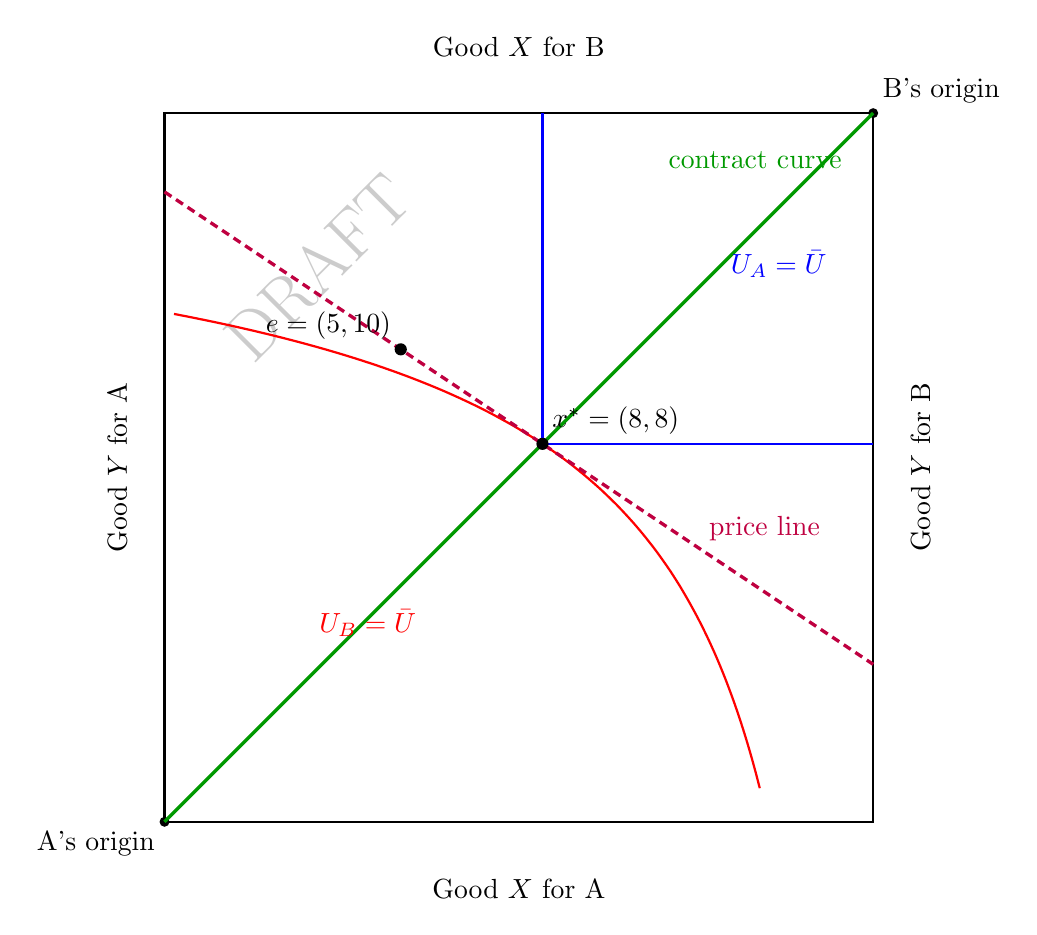
\begin{tikzpicture}[x=0.60cm,y=0.60cm]
      % Edgeworth box
      \draw[thick] (0,0) rectangle (15,15);

      % Origins
      \fill (0,0) circle (1.8pt);
      \fill (15,15) circle (1.8pt);
      \node[below left] at (0,0) {A's origin};
      \node[above right] at (15,15) {B's origin};

      % Axis labels
      \node[below] at (7.5,-1.0) {Good \(X\) for A};
      \node[rotate=90] at (-1.0,7.5) {Good \(Y\) for A};
      \node[above] at (7.5,16.0) {Good \(X\) for B};
      \node[rotate=90] at (16.0,7.5) {Good \(Y\) for B};

      % A indifference curves (Leontief)
     
      \draw[blue, thick] (8,8) -- (8,15);
      \draw[blue, thick] (8,8) -- (15,8);


      % B indifference curves in A-coordinates
      % (15-x_A)^{0.4}(15-y_A)^{0.6}=c
    
      \draw[red, thick, domain=0.2:12.6, samples=140, smooth]
        plot (\x,{15-((7)/((15-\x)^0.4))^(1/0.6)});

      % Contract curve x_A = y_A
      \draw[green!60!black, very thick] (0,0) -- (15,15);

      % Budget line through endowment and equilibrium
      \draw[purple, densely dashed, very thick] (0,13.333) -- (15,3.333);

      % Endowment and equilibrium
      \fill (5,10) circle (2.2pt) node[above left] {$e=(5,10)$};
      \fill (8,8) circle (2.2pt) node[above right] {$x^*=(8,8)$};

      % Labels
      \node[blue] at (13.0,11.8) {$U_A=\bar U$};
      \node[red] at (4.3,4.2) {$U_B=\bar U$};
      \node[green!60!black] at (12.5,14.0) {contract curve};
      \node[purple] at (12.7,6.2) {price line};
    \end{tikzpicture}
    \end{center}

    \item
    Consider the feasible allocation
    \[
    (x_A,y_A)=(7,7),
    \]
    so B receives
    \[
    (x_B,y_B)=(8,8).
    \]

    To show that \((7,7)\) is Pareto efficient, note first that A's utility is
    \[
    U_A(7,7)=7.
    \]
    For A to be at least as well off after any reallocation, we must have
    \[
    x_A'\ge 7
    \qquad\text{and}\qquad
    y_A'\ge 7,
    \]
    because
    \[
    \min\{x_A',y_A'\}\ge 7.
    \]

    Since the total endowment is \((15,15)\), this means B can receive at most
    \[
    (15-7,\;15-7)=(8,8).
    \]
    But B already receives \((8,8)\) at the candidate allocation. Since B's preferences are strictly increasing, there is no feasible way to make B strictly better off while keeping A at least as well off. Hence \((7,7)\) is Pareto efficient.

    Therefore
    \[
    \boxed{(7,7)\text{ is Pareto efficient.}}
    \]

    Now provide an initial endowment different from \((7,7)\) that supports this allocation as a competitive equilibrium.

    Use the same equilibrium prices as in part (a):
    \[
    p_X=\frac{2}{3},\qquad p_Y=1.
    \]

    For A to choose \((7,7)\), A must have income
    \[
    m_A= p_X\cdot 7 + 1\cdot 7
    = \frac{14}{3}+7
    = \frac{35}{3}.
    \]
    So we need an endowment \(\omega_A=(a,b)\) satisfying
    \[
    \frac{2}{3}a+b=\frac{35}{3},
    \]
    but \((a,b)\neq(7,7)\).

    One convenient choice is
    \[
    \boxed{\omega_A=(1,11).}
    \]
    Then B's endowment is
    \[
    \boxed{\omega_B=(14,4).}
    \]
    Check A's wealth:
    \[
    \frac{2}{3}\cdot 1 + 11 = \frac{2}{3}+\frac{33}{3}=\frac{35}{3},
    \]
    so A demands \((7,7)\).

    B's wealth is
    \[
    \frac{2}{3}\cdot 14 + 4 = \frac{28}{3}+\frac{12}{3}=\frac{40}{3}.
    \]
    With Cobb--Douglas utility,
    \[
    x_B=\frac{0.4(40/3)}{2/3}=8,
    \qquad
    y_B=0.6\left(\frac{40}{3}\right)=8.
    \]
    So B demands \((8,8)\).

    Thus, starting from the endowment
    \[
    \boxed{\omega_A=(1,11),\qquad \omega_B=(14,4),}
    \]
    the competitive equilibrium allocation after trade is exactly
    \[
    \boxed{A:(7,7),\qquad B:(8,8).}
    \]

    \item
    Interpreting \emph{fair} as \emph{envy-free}, the statement is \textbf{False}.

    A competitive equilibrium is always Pareto efficient under the standard assumptions, but it need not be envy-free. It depends on the initial endowments.

    A counterexample is given by this same economy with the original endowments:
    \[
    \omega_A=(5,10),\qquad \omega_B=(10,5).
    \]
    From part (a), the competitive equilibrium allocation is
    \[
    A:(8,8),\qquad B:(7,7).
    \]

    Check envy:
    \[
    U_A(8,8)=8,
    \qquad
    U_A(7,7)=7,
    \]
    so A does not envy B.

    But
    \[
    U_B(7,7)=7^{0.4}7^{0.6}=7,
    \]
    while
    \[
    U_B(8,8)=8^{0.4}8^{0.6}=8.
    \]
    So B strictly prefers A's bundle to his own, and therefore B envies A.

    Hence this competitive equilibrium is not fair. Therefore
    \[
    \boxed{\text{False.}}
    \]
\end{enumerate}
\end{document}